%%%%%%%%%%%%%%%%%%%%%%%%%%%%%%%%%%%%%%%%%%%%%%%%%%%
%% LaTeX book template                           %%
%% Author:  Amber Jain (http://amberj.devio.us/) %%
%% License: ISC license                          %%
%%%%%%%%%%%%%%%%%%%%%%%%%%%%%%%%%%%%%%%%%%%%%%%%%%%

\documentclass[a4paper,11pt,oneside]{book}

% pacotes utilizados
\usepackage[T1]{fontenc}
\usepackage[utf8]{inputenc}
\usepackage{lmodern}
\usepackage{hyperref}
\usepackage{graphicx}
\usepackage[portuguese]{babel}
\usepackage{amsfonts}
\usepackage[usenames,dvipsnames]{xcolor}
\usepackage{mathtools}
\usepackage{amssymb} % alguns simbolos matematicos
\usepackage{mathrsfs} % letras cursivas
\usepackage{listings} % coding examples in latex file
\usepackage{xcolor} % changing colors
\usepackage{amsthm} % definir estilo do teorema
\usepackage[hang,flushmargin]{footmisc} % remove footnote's identation
\usepackage{cancel} % para poder colocar o tracinho de cancelamento
\usepackage{tikz} % to draw Venn's diagrams
\usepackage{amsmath} % to write a function by cases
\usepackage{graphicx} % to set a images directory
\usepackage{caption} % to supress numbering in figures
\usepackage{float} % to make a figure stay when i whant

\graphicspath{{./images/}} % set an default images folder

% dark theme no pdf
\pagecolor[rgb]{0.1,0.1,0.1} %black
\color[rgb]{0.9,0.9,0.9} %grey

% criando o modelo de definicoes/teoremas/fatos/demonstracoes
\theoremstyle{definition}

\newtheoremstyle{break}% name
  {10pt}%         Space above, empty = `usual value'
  {10pt}%         Space below
  {}% Body font
  {}%         Indent amount (empty = no indent, \parindent = para indent)
  {\bfseries}% Thm head font
  {}%        Punctuation after thm head
  {\newline}% Space after thm head: \newline = linebreak
  {}%         Thm head spec

\theoremstyle{break}

% definindo as categorias de formalidade
\newtheorem{definition}{Definição}[section]
\newtheorem{fact}{Fato}[section]
\newtheorem{demonstration}{Demonstração}[section]
\newtheorem{theorem}{Teorema}

% tirando identação dos paragrafos
\setlength{\parindent}{0ex}

% setting das cores quando usar codigo python
\definecolor{codegreen}{rgb}{0,0.6,0}
\definecolor{codegray}{rgb}{0.5,0.5,0.5}
\definecolor{codepurple}{rgb}{0.58,0,0.82}
\definecolor{backcolour}{rgb}{0.95,0.95,0.92}

\lstdefinestyle{mystyle}{
    backgroundcolor=\color{backcolour},   
    commentstyle=\color{codegreen},
    keywordstyle=\color{magenta},
    numberstyle=\tiny\color{codegray},
    stringstyle=\color{codepurple},
    basicstyle=\ttfamily\footnotesize,
    breakatwhitespace=false,         
    breaklines=true,                 
    captionpos=b,                    
    keepspaces=true,                 
    numbers=left,                    
    numbersep=5pt,                  
    showspaces=false,                
    showstringspaces=false,
    showtabs=false,                  
    tabsize=2
}

\lstset{style=mystyle}

% dedicatoria 
% Source: http://www.tug.org/pipermail/texhax/2010-June/
\newenvironment{dedication}
{
   \cleardoublepage
   \thispagestyle{empty}
   \vspace*{\stretch{1}}
   \hfill\begin{minipage}[t]{0.66\textwidth}
   \raggedright
}
{
   \end{minipage}
   \vspace*{\stretch{3}}
   \clearpage
}

% Chapter quote at the start of chapter        %
% Source: http://tex.stackexchange.com/a/53380 %
\makeatletter
\renewcommand{\@chapapp}{}% Not necessary...
\newenvironment{chapquote}[2][2em]
  {\setlength{\@tempdima}{#1}%
   \def\chapquote@author{#2}%
   \parshape 1 \@tempdima \dimexpr\textwidth-2\@tempdima\relax%
   \itshape}
  {\par\normalfont\hfill--\ \chapquote@author\hspace*{\@tempdima}\par\bigskip}
\makeatother


%%%%%%%%%%%%%%%%%%%%%%%%%%%%%%%%%%%%%%%%%%%%%%%%%%%
% First page of book which contains 'stuff' like: %
%  - Book title, subtitle                         %
%  - Book author name                             %
%%%%%%%%%%%%%%%%%%%%%%%%%%%%%%%%%%%%%%%%%%%%%%%%%%%
% Book's title and subtitle
\title{\Huge \textbf{Microeconomia} \\ 
\Large Tradução da 9 edição \\
\huge Hal R. Varian}

% Author
\author{
\textsc{Resumo e Adaptação por:} \\
\textsc{Bruno de M. Ruas}
}

\begin{document}

\frontmatter
\maketitle

\tableofcontents
%\listoffigures
%\listoftables

\mainmatter

%%%%%%%%%%%%%%%%%%%%%%%% PART %%%%%%%%%%%%%%%%%%%%%%%%
\part*{Preparativos}
\addcontentsline{toc}{part}{Preparativos}

%%%%%%%%%%%%%%%%%%%%%%%% CHAPTER %%%%%%%%%%%%%%%%%%%%%%%%
\chapter*{Matemática}
\addcontentsline{toc}{chapter}{Matemática}

\begin{chapquote}{The Godfather}
	``Some Day, And That Day May Never Come, I Will Call Upon You To Do A Service For Me.''.
\end{chapquote}

Bem vindo ao meu resumo do livro do prof. Varian. Ao contrário do que ele fez, eu preferi trazer o apêndice de matemática pro começo do material porque aqui nós vamos ver as ferramentas que serão usadas para a explicação dos conceitos teóricos ao longo do material.
\\
\\
Aqui a gente só vai dar um overview básico nos conceitos. Não tenha dúvida que alguém mais experimentado em matemática torceria o nariz pra algumas definições dadas aqui. Mas o objetivo é te dar um "norte"\ a respeito de alguns conceitos normalmente usados. Não se assuste com a simplicidade de algumas coisas. Melhor garantir agora do que sofrer mais pra frente no texto.

\section*{Funções}
\addcontentsline{toc}{section}{Funções}

Sejam dois números quaisquer $x$ e $y$, uma \textbf{função} ou \textbf{transformação} é uma regra que descreve uma relação entre eles.
\\
\\
Para demonstrar que existe alguma dependência entre duas variáveis usamos a notação $y = f(x)$, onde nossa variável $y$ (chamada de \textbf{dependente}) é o resultado de alguma transformação (denotada pelo símbolo $"f"$) realizada em $x$ (nossa variável \textbf{independente}).
\\
\\
Não é raro ter uma variável dependente relacionada a várias outras variáveis. Nesses casos é comum o uso da notação anterior com a adição das novas incógnitas. Algo como $y = f(x_1,x_2,...,x_n)$.

\section*{Gráficos}
\addcontentsline{toc}{section}{Gráficos}

Não tem muito o que falar aqui. Dá uma lida lá na página 1010.

\section*{Propriedades das Funções}
\addcontentsline{toc}{section}{Propriedades das Funções}

Uma função pode ter algumas características que facilitam a sua descrição. Aqui temos algumas que serão usadas ao longo do curso:
\\
\\
Uma \textbf{função contínua} é aquela que não possui nenhum "salto"\ ou "quebra". 
\\
\\
Uma \textbf{função suave} é aquela que não tem "dobras"\ nem "cantos".
\\
\\
Uma \textbf{função monotônica} é aquela que sempre segue o mesmo sentido (ou crescendo ou decrescendo) sem nunca mudar de sentido. 
Quando é crescente a medida que $x$ cresce, chamaremos de \textbf{função monotônica crescente}. Quando decrescer a medida que $x$ crescer, chamaremos de \textbf{função monotônica decrescente}.

\section*{Funções Inversas}
\addcontentsline{toc}{section}{Funções Inversas}

Uma das implicações de quando uma função é monotônica é que, para cada $x$, sempre existirá apenas um único $y$ associado. 
\\
\\
Uma \textbf{função inversa} é a função que, sempre que colocarmos um $y$ como variável independente teremos como resultado um $x$ de alguma função anterior.\footnote{Eu tentei não deixar confuso mas se ficou com dúvida, pesquisa um pouco sobre o tema.}

\section*{Equações e Identidades}
\addcontentsline{toc}{section}{Equações e Identidades}

Podemos relacionar dois ou mais elementos por meio do uso de \textbf{equações} (usando o símbolo da igualdade "$=$"). Onde as suas respectivas \textbf{soluções} são os valores atribuíveis as incógnitas que assegurem a validade da relação proposta.
\\
\\
Uma \textbf{identidade} (que tem o símbolo dado por "$\equiv$") é um tipo de relação onde sempre haverá as soluções independentemente de quais valores suas variáveis assumam.

\section*{Funções Lineares}
\addcontentsline{toc}{section}{Funções Lineares}

Chamamos de \textbf{função linear}, qualquer função da forma $y = ax + b$. Fique atento porque uma função linear pode ser expressa de maneira implícita (ou seja, será necessário desenvolver um pouco a álgebra até que se chegue numa equação no formato da definição).

\section*{Variações e Taxas de Variação}
\addcontentsline{toc}{section}{Variações e Taxas de Variação}

Usamos o símbolo "$\Delta$"\footnote{O nome é "delta".} para denotar a variação de alguma variável. Ou seja, se tivemos uma variável qualquer $x$ que teve seu valor alterado de $x^1$ para $x^2$, então:

$$ \Delta x = x^2 - x^1 $$
ou também
$$ x^2 = x^1 + \Delta x $$
\\
Normalmente, usamos o delta quando falamos de \textbf{pequenas variações} ou, como os economistas falam, \textbf{variações marginais}.
\\
\\
A \textbf{taxa de variação} é obtida pela razão (ou seja, pela divisão) de duas variações. Seja a função $y = f(x)$, sempre que tivemos um $\Delta x > 0$ também teremos algum $\Delta y \neq 0$. A taxa de variação de $y$ em relação à $x$ é dada por:

$$ \frac{\Delta y}{\Delta x} = \frac{y^2 - y^1}{x^2 - x^1} = \frac{f(x^1 + \Delta x) - f(x^1)}{\Delta x} $$
\\
É uma medida do quanto $y$ varia a medida que $x$ varia.
\\
\\
Quando uma função é linear, teremos que essa taxa de variação será sempre constante para quaisquer valores de $x$. Como $y = ax + b$, então
\\
\\
\Large $ \frac{\Delta y}{\Delta x} = $ \normalsize
$$ \frac{a+b(x^1 + \Delta x) - (a + bx^1)}{\Delta x} = $$
$$ \frac{\cancel{a}+b(x^1 + \Delta x) \cancel{-a} - bx^1)}{\Delta x} = $$
$$ \frac{\cancel{bx^1} + b \Delta x \cancel{- bx^1}}{\Delta x} = $$
$$ \frac{b \cancel{\Delta x}}{\cancel{\Delta x}} = b  $$

Para as funções não lineares, essa propriedade não é observada. Tomemos $y = f(x) = x^2$ como exemplo,
\\
\\
\Large $ \frac{\Delta y}{\Delta x} = $ \normalsize
$$ \frac{(x + \Delta x)^2 - x^2}{\Delta x} = $$ 
$$  \frac{\cancel{x^2} + 2x \Delta x + (\Delta x)^2 \cancel{-x^2}}{\Delta x} = $$
$$  \frac{2x \cancel{\Delta x} + \Delta x . \cancel{\Delta x}}{\cancel{\Delta x}} = $$
$$  2x + \Delta x $$
\\
Ou seja, entra no resultado da taxa de variação o valor de $x$ e a magnitude da variação, dada por $\Delta x$.

\section*{Inclinações e Interceptos}
\addcontentsline{toc}{section}{Inclinações e Interceptos}

Já aprendemos como calcular a taxa de variação de uma função. Graficamente falando, essa é a medida da inclinação da curva da função entre os dois pontos que formam o delta da variável independente. 
\\
\\
Em uma função linear, a inclinação da curva sempre será a mesma independente da magnitude da variação. No caso das funções não lineares, a inclinação é dada pela \textbf{reta tangente} ao ponto da curva\footnote{Mais pra frente a gente volta nessa ideia.}.
\\
\\
No caso de uma função linear, $ y = ax + b$, temos alguns pontos que recebem nomes de \textbf{intercepto}. O \textbf{intercepto vertical} ($y^*$) é dado pelo ponto $y = a.0 + b = b$, ou seja, onde $x = 0$. Já o \textbf{intercepto horizontal} ($x^*$) é dado pelo ponto onde $y = ax + b = 0 $, ou seja, $ x = \frac{-b}{a}$.

\section*{Valores absolutos e logaritmos}
\addcontentsline{toc}{section}{Valores Absolutos e Logaritmos}

O \textbf{valor absoluto} de um número $x$ qualquer é definido pela função $f(x)$ do seguinte modo:

\[ f(x) = |x| = \begin{cases} x & se \ x \geqslant \\ -x & se \ x < 0 \end{cases} \]
\\
\\
Você já deve ter visto no ensino médio que o \textbf{logaritmo natural} ou \textbf{log} de um número é uma função escrita como $y = lnx$ ou $y = ln(x)$ e que possui as seguintes propriedades:

\begin{itemize}
 \item Se $x,y > 0$, então, $ ln(xy) = ln(x) + ln(y) $
 \item $ ln(e) = 1 $
 \item $ ln(x^y) = y ln(x) $
\end{itemize}

\section*{Derivadas}
\addcontentsline{toc}{section}{Derivadas}

Você deve lembrar desse conceito das aulas de matemática no primeiro período. A \textbf{derivada} da função $f(x)$ será dada por:

$$ f'(x) = \frac{df(x)}{dx} = \lim_{\Delta x \to 0} \frac{f(x + \Delta x) - f(x)}{\Delta x} $$
\\
Mas perai, a gente acabou de ver um conceito muito parecido no ponto 1.7. E é isso mesmo, a derivada é o cálculo da taxa de variação à medida que aplicamos o limite\footnote{Vá pesquisar se você não souber o que é isso.} até $0$ para nosso $\Delta x$.
\\
\\
\textbf{Comentário}: Essa técnica é muito importante ao longo de quase todos os tópicos desse curso. Volte nas apostilas e nas listas de derivadas caso seja necessário.

\section*{Derivadas segundas}
\addcontentsline{toc}{section}{Derivadas Segundas}

Já vimos que a deriva nos permite saber a inclinação da reta tangente da nossa função genérica $f(x)$ num determinado ponto. Chamamos de \textbf{derivada segunda} de $f(x)$ a derivada da derivada dessa função.

$$ f''(x) = \frac{d^2f(x)}{dx^2} $$
\\
Nós aplicamos a derivada segunda para descobrirmos a curvatura da função no ponto $x$. Se for positiva, a função é convexa no ponto. Se for negativa, a função é côncava no ponto. Por fim, se for igual a zero, a função será plana.

\section*{A regra do produto e da cadeia}
\addcontentsline{toc}{section}{A regra do Produto e da Cadeia}

Dadas duas funções $g(x)$ e $h(x)$ Se definirmos uma nova função $f(x) = g(x) h(x)$. A derivada dessa última função é dada pela aplicação da \textbf{regra do produto}:
\\
$$ \frac{df(x)}{dx} = g(x)\frac{dh(x)}{dx} + h(x)\frac{dg(x)}{dx}$$
\\
\\
\textbf{Comentário}: Normalmente a gente vê a regra do produto e da divisão junto. Mas o prof. Varian não colocou essa segunda regra como necessária. Então se eu ver que ficou faltando, eu atualizo esse material.
\\
\\
Agora imagine a situação onde temos uma função dentro de outra função. Dadas as funções $y = g(x)$ e $z = h(y)$, a \textbf{função composta} é dada por $f(x) = h(g(x))$, cuja derivada é obtida pela seguinte regra:

$$ \frac{df(x)}{dx} = \frac{dh(y)}{dy}\frac{dg(x)}{x}$$

\section*{Derivadas parciais}
\addcontentsline{toc}{section}{Derivadas Parciais}

Nós já vimos no ponto 1.1 que funções podem conter mais de uma variável independente. Supondo uma função composta $f(x_1,x_2)$ a sua \textbf{derivada parcial} em relação a $x_1$ será dada por:

$$ \frac{\partial f(x_1,x_2)}{\partial x_1} = 
\lim_{\Delta x_1 \to 0} \frac{f(x_1+\Delta x_1,x_2) - f(x_1,x_2)}{\Delta x_1} $$
\\
similarmente, a derivada parcial em relação a $x_2$ será dada por
\\
$$ \frac{\partial f(x_1,x_2)}{\partial x_2} = 
\lim_{\Delta x_2 \to 0} \frac{f(x_1,x_2+\Delta x_2) - f(x_1,x_2)}{\Delta x_2} $$
\\
A ideia por trás de uma derivada parcial é verificar a taxa de variação entre a nossa função composta em relação a alguma variação de apenas uma das variáveis independentes, ou seja, é como se tratássemos as outras variáveis como constantes.
\\
\\
As propriedades das derivadas parciais são parecidas com as normais. Exceção é a regra da cadeia. Seja a função composta $g(t) = f(x_1(t),x_2(t))$, então a derivada de $g(t)$ em relação a $t$ é dada por:

$$ \frac{dg(t)}{dt} = 
\frac{\partial f(x_1,x_2)}{\partial x_1}\frac{dx_1(t)}{dt} + 
\frac{\partial f(x_1,x_2)}{\partial x_2}\frac{dx_2(t)}{dt} $$
\\
Atente para o fato que as variáveis independentes da nossa função $g(t)$ são as funções $x_1(t)$ e $x_2(t)$ que também têm como variável independente $t$.

\section*{Otimização}
\addcontentsline{toc}{section}{Otimização}

A maioria dos modelos utilizados pela Economia podem ser expressos como um problemas de otimização. Matematicamente falando, dada uma função $y = f(x)$ seu valor \textbf{máximo} será dado ponto $x^*$ se $f(x^*) \geqslant f(x)$ para qualquer valor de $x$. Não faz parte do escopo desse apêndice demonstrar isso, então tenha fé que, se uma função for suave, o seu valor máximo é obtido no ponto onde teremos

$$ \frac{df(x^*)}{dx} = 0 $$

e também

$$ \frac{d^2f(x^*)}{dx^2} \leq 0$$
\\
Ou seja, o máximo será o ponto onde a derivada for igual a zero e a derivada segunda for menor igual a zero. Chamamos a primeira de \textbf{condição de primeira ordem} e a segunda de \textbf{condição de segunda ordem}.
\\
\\
Também é muito comum buscarmos a minimização de determinadas funções. Nesse caso, só teremos uma pequena mudança na condição de segunda ordem;

$$ \frac{df(x^*)}{dx} = 0 $$

e também

$$ \frac{d^2f(x^*)}{dx^2} \geq 0$$
\\
No casos das funções compostas suaves, as condições de primeira ordem para os pontos de máximo e mínimo são alcançadas no ponto $(x_{1}^*,x_{2}^*)$ cujas derivadas serão

$$ \frac{\partial f(x_{1}^*,x_{2}^*)}{\partial x_1} = 0 $$
e
$$ \frac{\partial f(x_{1}^*,x_{2}^*)}{\partial x_2} = 0 $$
\\
As condições de segunda ordem são muito mais complexas então não fazem parte do escopo desse curso.

\section*{Otimização com restrição}
\addcontentsline{toc}{section}{Otimização com Restrição}

Saber maximizar ou minimizar uma função é só uma parte do problema de otimização. Na vida real, a esmagadora maioria das situações de otimização está contida dentro de algum limite de possibilidades. A \textbf{otimização com restrição} é a técnica usada para encontrar o ponto de máximo ou mínimo de alguma função dentro de um determinado domínio de possibilidades.

\begin{center}
\LARGE $\stackrel{máx}{\text{\small $x_1,x_2$}} \ \ \stackrel{f(x_1,x_2)}{\ }$ \\
\normalsize $\textrm{de modo que } g(x_1,x_2) = c$
\end{center}

A função $f(x_1,x_2)$ é chamada de \textbf{função objeto} e a equação $g(x_1,x_2) = c$ é chamada de \textbf{restrição}.

%%%%%%%%%%%%%%%%%%%%%%%% CHAPTER %%%%%%%%%%%%%%%%%%%%%%%%
\chapter*{Programação}
\addcontentsline{toc}{chapter}{Programação}

\begin{chapquote}{The Godfather}
	``I don’t like violence, Tom. I’m a businessman. Blood is a big expense.''.
\end{chapquote}


Caro aluno, com o avanço do poder computacional e da disponibilidade de dados, os economistas não ficaram de fora da revolução tecnológica. Além de todo o arcabouço teórico, matemático, estatístico, histórico e social que você está adquirindo na sua formação, a programação se tornou uma ferramenta indispensável para o processo de análise moderna e merece ser objeto do seu estudo\footnote{Pode até ser que você não tenha alguma matéria de programação na sua grade curricular, mas não se engane, mesmo que seu curso não esteja cobrando, vá estudar por conta própria.}.
\\
\\
Ao longo do livro eu vou construir alguns programas em Python para simular os modelos que a gente for construindo. Não faz parte do escopo desse livro ensinar como fazer isso. Contudo, cada código será disponibilizado em dois links. O primeiro é referente ao repositório no github e o segundo é referente a um notebook no google colab onde você pode executar o modelo sem precisar instalar nada no seu computador.

\section*{Capítulo 25 - Monopólio}
\addcontentsline{toc}{section}{Capítulo 25 - Monopólio}

\subsection*{Demanda Linear e Monopólio (25.2)}
\addcontentsline{toc}{subsection}{Demanda Linear e Monopólio (25.2)}

\begin{center}
\href{https://github.com/brunoruas2/Meus_Estudos/blob/main/Microeconomia/Microeconomics\%20-\%20Hal\%20Varian/models/cap25.2-demanda_linear_e_monopolio.py}{
\includegraphics[scale=0.03]{_github_logo.png} \ Código no Github \ 
\includegraphics[scale=0.03]{_github_logo.png}}
\\
\ 
\\
\href{https://colab.research.google.com/drive/1OUK3Z--dv7WMufCLmJ9qDWII1yoVlWVX?usp=sharing}{
\includegraphics[scale=0.08]{_colab_logo.png} Simulação no Google Colab 
\includegraphics[scale=0.08]{_colab_logo.png}}
\end{center}

\subsection*{Demanda Elasticidade Constante e Monopólio (25.3)}
\addcontentsline{toc}{subsection}{Demanda Elasticidade Constante e Monopólio (25.3)}

\begin{center}
\href{https://github.com/brunoruas2/Meus_Estudos/blob/main/Microeconomia/Microeconomics\%20-\%20Hal\%20Varian/models/cap25.3-demanda_ces_e_monopolio.py}{
\includegraphics[scale=0.03]{_github_logo.png} \ Código no Github 
\includegraphics[scale=0.03]{_github_logo.png}}
\\
\ 
\\
\href{https://colab.research.google.com/drive/1MRJb9DZ7n_Hz2Kp9ng8K7pOcb1DTy_u5?usp=sharing}{
\includegraphics[scale=0.08]{_colab_logo.png} Simulação no Google Colab 
\includegraphics[scale=0.08]{_colab_logo.png}}
\end{center}


\section*{Capítulo 26 - Comportamento do Monopolista}
\addcontentsline{toc}{section}{Capítulo 26 - Comportamento do Monopolista}

\subsection*{Demandas Lineares e Discriminação de Preço (26.4)}
\addcontentsline{toc}{subsection}{Demandas Lineares e Discriminação de Preço (26.4)}

\begin{center}
\href{https://github.com/brunoruas2/Meus_Estudos/blob/main/Microeconomia/Microeconomics\%20-\%20Hal\%20Varian/models/varian_26.5_vinculacao_produtos.ipynb}{
\includegraphics[scale=0.03]{_github_logo.png} \ Código no Github 
\includegraphics[scale=0.03]{_github_logo.png}}
\\
\ 
\\
\href{https://drive.google.com/file/d/10zbnTsvdiLaHEYt3q8ShhJlkW7q1QVzG/view?usp=sharing}{
\includegraphics[scale=0.08]{_colab_logo.png} Simulação no Google Colab 
\includegraphics[scale=0.08]{_colab_logo.png}}
\end{center}

\subsection*{Vinculação de Produtos (26.5)}
\addcontentsline{toc}{subsection}{Vinculação de Produtos (26.5)}

\begin{center}
\href{https://github.com/brunoruas2/Meus_Estudos/blob/main/Microeconomia/Microeconomics\%20-\%20Hal\%20Varian/models/varian_26.5_vinculacao_produtos.ipynb}{
\includegraphics[scale=0.03]{_github_logo.png} \ Código no Github 
\includegraphics[scale=0.03]{_github_logo.png}}
\\
\ 
\\
\href{https://drive.google.com/file/d/1WhxGaAhUB9dKkgrKWadihIrzS4cm3bXP/view?usp=sharing}{
\includegraphics[scale=0.08]{_colab_logo.png} Simulação no Google Colab 
\includegraphics[scale=0.08]{_colab_logo.png}}
\end{center}

%%%%%%%%%%%%%%%%%%%%%%%% PART %%%%%%%%%%%%%%%%%%%%%%%%
\part{Teoria da Escolha e Teoria do Consumidor}

%%%%%%%%%%%%%%%%%%%%%%%% CHAPTER %%%%%%%%%%%%%%%%%%%%%%%%
\chapter{O Mercado}

\begin{chapquote}{The Godfather}
	``A friend should always underestimate your virtues and an enemy overestimate your faults.''
\end{chapquote}

%\section{A elaboração de um modelo}
%\section{Otimização e equilíbrio}
%\section{A curva de demanda}
%\section{A curva de oferta}
%\section{O equilíbrio de mercado}
%\section{A estática comparativa}
%\section{Outras formas de alocar apartamentos}
%\section{Qual o melhor arranjo?}
%\section{A eficiência de Pareto}
%\section{Comparação entra as formas de alocação de apartamentos}
%\section{Equilíbrio no longo prazo}

%%%%%%%%%%%%%%%%%%%%%%%% CHAPTER %%%%%%%%%%%%%%%%%%%%%%%%
\chapter{Restrição Orçamentária}

%%%%%%%%%%%%%%%%%%%%%%%% CHAPTER %%%%%%%%%%%%%%%%%%%%%%%%
\chapter{Preferências}

%%%%%%%%%%%%%%%%%%%%%%%% CHAPTER %%%%%%%%%%%%%%%%%%%%%%%%
\chapter{Utilidade}

%%%%%%%%%%%%%%%%%%%%%%%% CHAPTER %%%%%%%%%%%%%%%%%%%%%%%%
\chapter{Escolha}

%%%%%%%%%%%%%%%%%%%%%%%% CHAPTER %%%%%%%%%%%%%%%%%%%%%%%%
\chapter{Demanda}

%%%%%%%%%%%%%%%%%%%%%%%% CHAPTER %%%%%%%%%%%%%%%%%%%%%%%%
\chapter{Preferência Revelada}

%%%%%%%%%%%%%%%%%%%%%%%% CHAPTER %%%%%%%%%%%%%%%%%%%%%%%%
\chapter{A Equação de Slutsky}

%%%%%%%%%%%%%%%%%%%%%%%% CHAPTER %%%%%%%%%%%%%%%%%%%%%%%%
\chapter{Comprando e Vendendo}

%%%%%%%%%%%%%%%%%%%%%%%% CHAPTER %%%%%%%%%%%%%%%%%%%%%%%%
\chapter{Escolha Intertermporal}

%%%%%%%%%%%%%%%%%%%%%%%% CHAPTER %%%%%%%%%%%%%%%%%%%%%%%%
\chapter{Mercado de Ativos}

%%%%%%%%%%%%%%%%%%%%%%%% CHAPTER %%%%%%%%%%%%%%%%%%%%%%%%
\chapter{Incerteza}

%%%%%%%%%%%%%%%%%%%%%%%% CHAPTER %%%%%%%%%%%%%%%%%%%%%%%%
\chapter{Ativos de Risco}

%%%%%%%%%%%%%%%%%%%%%%%% CHAPTER %%%%%%%%%%%%%%%%%%%%%%%%
\chapter{O Excedente do Consumidor}

%%%%%%%%%%%%%%%%%%%%%%%% CHAPTER %%%%%%%%%%%%%%%%%%%%%%%%
\chapter{Demanda de Mercado}

%%%%%%%%%%%%%%%%%%%%%%%% PART %%%%%%%%%%%%%%%%%%%%%%%%
\part{Equilíbrio, Econometria e Leilões}

%%%%%%%%%%%%%%%%%%%%%%%% CHAPTER %%%%%%%%%%%%%%%%%%%%%%%%
\chapter{Equilíbrio}

%%%%%%%%%%%%%%%%%%%%%%%% CHAPTER %%%%%%%%%%%%%%%%%%%%%%%%
\chapter{Medição}

%%%%%%%%%%%%%%%%%%%%%%%% CHAPTER %%%%%%%%%%%%%%%%%%%%%%%%
\chapter{Leilões}

%%%%%%%%%%%%%%%%%%%%%%%% PART %%%%%%%%%%%%%%%%%%%%%%%%
\part{Teoria da Firma}

%%%%%%%%%%%%%%%%%%%%%%%% CHAPTER %%%%%%%%%%%%%%%%%%%%%%%%
\chapter{Tecnologia}

%%%%%%%%%%%%%%%%%%%%%%%% CHAPTER %%%%%%%%%%%%%%%%%%%%%%%%
\chapter{Maximização do Lucro}

%%%%%%%%%%%%%%%%%%%%%%%% CHAPTER %%%%%%%%%%%%%%%%%%%%%%%%
\chapter{Minimização de Custos}

%%%%%%%%%%%%%%%%%%%%%%%% CHAPTER %%%%%%%%%%%%%%%%%%%%%%%%
\chapter{Curva de Custo}

%%%%%%%%%%%%%%%%%%%%%%%% CHAPTER %%%%%%%%%%%%%%%%%%%%%%%%
\chapter{Oferta da Empresa}

%%%%%%%%%%%%%%%%%%%%%%%% CHAPTER %%%%%%%%%%%%%%%%%%%%%%%%
\chapter{Oferta da Indústria}

%%%%%%%%%%%%%%%%%%%%%%%% PART %%%%%%%%%%%%%%%%%%%%%%%%
\part{Mercados e Concorrência Imperfeita}

%%%%%%%%%%%%%%%%%%%%%%%% CHAPTER %%%%%%%%%%%%%%%%%%%%%%%%
\chapter{Monopólio}

\begin{chapquote}{The Godfather}
	``I'm gonna make him an offer he can't refuse.''
\end{chapquote}

Anteriormente, fora demonstrado como a oferta pode ser construída da firma individual até a indústria competitiva. Nesse cenário, todos os ofertantes não possuem poder de interferir no preço e na quantidade de equilíbrio do mercado. Mas podemos pensar num caso muito diferente: Como seria o caso onde só exista uma empresa controlando toda a oferta?
\\
\\
Diferente dos casos anteriores, agora nós buscamos construir um modelo de tomada de decisão que leve em consideração a capacidade do monopolista de intervir diretamente no preço de modo a maximizar seus lucros totais.
\\
\\
Existem duas maneiras de enxergar esse problema. Podemos modelar como se o monopolista controlasse o preço e a demanda é quem definiria a quantidade. Ou, ao contrário, podemos modelar como se o monopolista definisse a quantidade a ser produzida e a demanda definiria o seu preço de equilíbrio para essa quantidade.
\\
\\
Independente do modelo, podemos ver que as abordagens são equivalentes. Por facilidade analítica vamos seguir a abordagem de definição da quantidade produzida.

\section{Maximização dos Lucros}

Como vimos nos capítulo 01, estamos diante de um problema de maximização. Sendo mais preciso, nós queremos maximizar o lucro do monopolista dado por $yp(y) - c(y)$ onde $p(y)$ é a demanda inversa\footnote{Lá do capítulo 15. É a função que indica qual deve ser o preço do bem para que seja demanda uma determinada quantidade.} para o mercado, $r(y) = yp(y)$ é a receita do monopolista e $c(y)$ é o custo de produção das $y$ unidades. Podemos resumir nosso problema como

\begin{center}
\LARGE $\stackrel{máx}{\text{\small $y$}} \ \ \stackrel{r(y) - c(y)}{\ }$ \\
\end{center}

A condição de otimização é evidente: A receita marginal deve ser igual ao custo marginal. Se a receita marginal for maior, bastaria aumentar a produção para aumentar os lucros. Se fosse menor, seria necessário reduzir a quantidade produzida afim de elevar o preço a um nível satisfatório. Algebricamente, temos que

$$ \textrm{RM = CMa} $$
$$ ou $$
$$ \frac{\Delta r}{\Delta y} = \frac{\Delta c}{\Delta y} $$
\\
Até aqui a gente tá bem perto da modelagem para as firmas competidoras. O custo marginal é definido pela tecnologia de produção. A mudança acontecerá na receita marginal. 
\\
\\
Como o monopolista tem o poder de intervir no mercado, sempre que ele decidir alterar a produção em $\Delta y$ unidades, haverá dois efeitos na receita. Em primeiro lugar, ele terá um aumento na receita em $p\Delta y$ unidades. Em segundo lugar, como o mercado terá mais bens a sua disposição, ele estará disposto a pagar um preço menor pelas novas unidades, ou seja, $y\Delta p$. O resultado líquido desse efeito é obtido por

$$\Delta r = p \Delta y + y \Delta p$$

$$ \frac{\Delta r}{\Delta y} = 
\frac{p \Delta y}{\Delta y} + 
\frac{y \Delta p}{\Delta y} $$

$$ \phantom{\frac{\Delta r}{\Delta y}} = 
\frac{p \cancel{\Delta y}}{\cancel{\Delta y}} + 
\frac{y \Delta p}{\Delta y} $$

$$ \phantom{\frac{\Delta r}{\Delta y}} = p + y\frac{\Delta p}{\Delta y} $$

$$ \phantom{\frac{\Delta r}{\Delta y}} = 
p \left[ 1 + \underbrace{\frac{y}{p}\frac{\Delta p}{\Delta y}}_\text{1/elasticidade} \right] $$

$$ \phantom{\frac{\Delta r}{\Delta y}} = 
p \left[ 1 + \frac{1}{\epsilon(y)} \right] $$
\\
Como a elasticidade da demanda é negativa, podemos reescrever como

$$ \frac{\Delta r}{\Delta y} = 
RM(y) =
p \left[ 1 - \frac{1}{|\epsilon(y)|} \right] $$
\\
Agora que sofisticamos um pouco mais a ideia da receita marginal. Voltemos para a condição de maximização onde a Receita Marginal deve ser igual a o Custo Marginal.

$$ p(y) \left[ 1 - \frac{1}{|\epsilon(y)|} \right] = CMa(y) $$
\\
Agora podemos ver claramente que o nosso monopolista atuará somente nos pontos onde a demanda é elástica ($|\epsilon| > 1$). Se operar no ponto onde $\epsilon = 1$, cairá exatamente no caso da competição perfeita\footnote{Onde o preço é igual ao custo marginal.}. Não faz sentido para ele operar nos pontos onde a demanda é inelástica porque ele poderia simplesmente reduzir a quantidade produzida (o que reduziria o custo total) com aumento de receita (porque o preço aumentaria). O ponto de máximo estará sempre na zona onde $|\epsilon| \geq 1$.

\section{Curva de Demanda Linear e Monopólio}

Veremos como fica o comportamento dessas variáveis num exemplo cuja curva de demanda é linear. O professor dá o seguinte sistema de equações:

$$ \textrm{Demanda Linear Inversa: } p(y) = a - by $$
$$ \textrm{Função Receita: } r(y) = p(y)y = ay - by^2 $$
$$ \textrm{Função Receita Marginal: } RM(y) = a - 2by $$
\\
A receita marginal é dada (como vemos no capítulo 15) pela derivada da função receita. Podemos ver que o intercepto vertical da demanda e da receita marginal são iguais (dado pelo ponto $a$).
\\
\\
\textbf{Simulação:} \href{https://colab.research.google.com/drive/1OUK3Z--dv7WMufCLmJ9qDWII1yoVlWVX?usp=sharing}{Clique aqui} para ter acesso a essa simulação. Você pode mudar os parâmetros de "$a$", "$b$", "CF"\ e "CV"\ afim de verificar como os valores se modificam.

\begin{center}
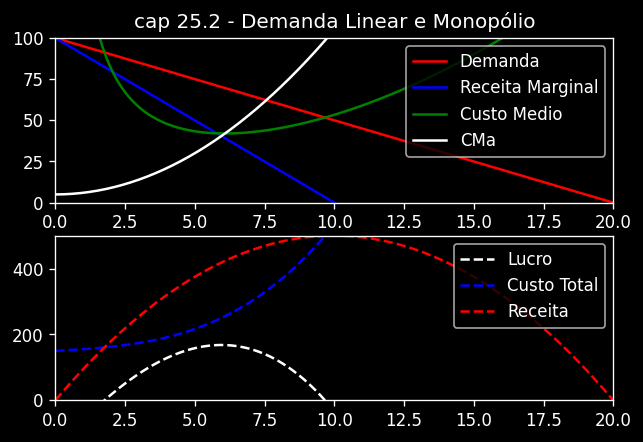
\includegraphics[scale=0.8]{cap25_2-demanda_linear_e_monopolio.png}
\end{center}

Para poder fazer essa simulação, eu tive de definir uma função custo e, consequentemente, uma função custo marginal\footnote{Eu tentei pensar numa função que apresentasse um comportamento parecido com a imagem que vemos no livro.}. Conseguimos ver que a curva de lucro tem um ponto de máximo exatamente onde a curva da receita marginal encontra o custo marginal. Qualquer ponto diferente desse levaria a um nível de lucro menor.
\\
\\
Além disso, também é relevante o fato da curva de custo médio estar abaixo da curva de demanda\footnote{Tente justificar isso matematicamente e, depois, tente criar uma situação onde isso acontece.}. Se o ponto de produção cuja receita marginal é igual ao custo marginal tiver um custo médio superior a demanda, a empresa receberá menos do que os custo de produção.\footnote{Veremos isso daqui a pouco no ponto 25.6.}.

\section{Estabelecimento de Preços com Markup}

Já conseguimos aprimorar nosso modelo de escolha da firma para o caso do monopolista. Agora que tornamos a receita marginal endógena, podemos ver as condições de maximização do lucro quando a firma tem poder de definir o preço ou a quantidade do mercado (mas não os dois ao mesmo tempo).
\\
\\
Podemos compreender essa última equação como uma política de preço do monopolista. Para isso, só precisamos isolar o termo $p(y)$ via rearranjo da última equação, o que após feito nos dá a seguinte relação

$$ p(y) = \frac{CMa(y)}{1 - 1/|\epsilon(y)|} $$
\\
Essa equação nos diz que o preço praticado no mercado cujo monopolista atua sempre\footnote{Sempre que ele agir de acordo com os pressupostos do nosso modelo de escolha.} se comportará como uma função de \textit{markup} do seu custo marginal. Podemos simplificar a visualização disso do seguinte modo

$$ p(y) = \phi \times CMa(y) $$
onde $\phi = \frac{1}{1 - 1/|\epsilon(y)|}$
\\
\\
Como sabemos, o monopolista sempre operará nos pontos cuja demanda é elástica\footnote{Ele até pode operar no ponto onde $\epsilon = 1$, já vimos que nesse caso, o resultado seria o mesmo do caso na competição perfeita.}, isso nos dará um $\epsilon(y) > 1$. Isso nos diz que o divisor $(1 - 1/|\epsilon|) <  1$, o que por sua vez, nos diz que $\phi > 1$.
\\
\\
Agora vamos dar uma olhada em um caso muito interessante: quando a curva de demanda possui a mesma elasticidade em todos os seus pontos.

\subsection{Demanda com Elasticidade Constante e Monopólio}

Para simular o caso da demanda com elasticidade constante, vamos usar o método do markup para encontrar o ponto de oferta do monopolista. Como esperado, teremos uma função de marcação acima da curva de custo marginal.

\begin{center}
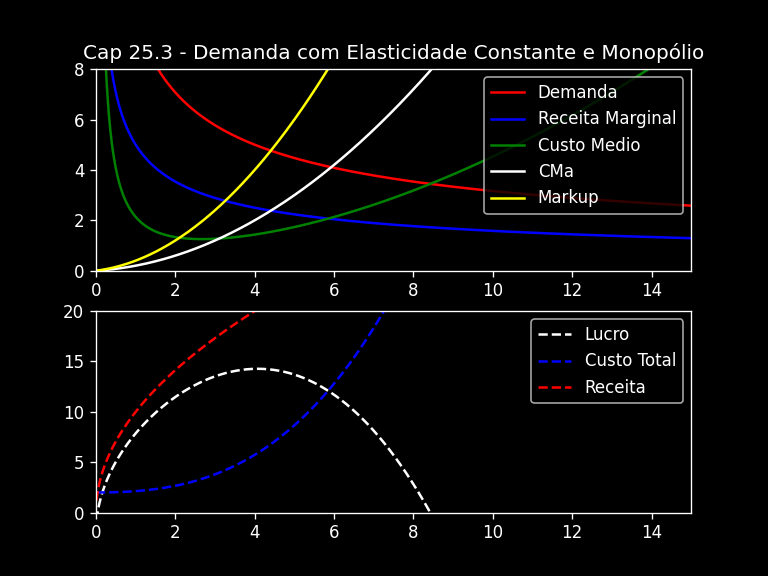
\includegraphics[scale=0.7]{cap25_3-demanda_ces_e_monopolio.png}
\end{center}

\textbf{Simulação:} \href{https://colab.research.google.com/drive/1MRJb9DZ7n_Hz2Kp9ng8K7pOcb1DTy_u5?usp=sharing}{Clique aqui} para ter acesso a essa simulação.
\\
\\
\textbf{Comentário:} Leia o exemplo sobre o impacto dos impostos sobre o monopolista na página 634. Com os conceitos vistos até agora, não deve ser difícil compreende-lo. Você pode acessar a simulação e modificar o custo variável para ver se o resultado é igual ao que você esperava.

\section{A Ineficiência do Monopólio}

Já conseguimos ver que, quando uma empresa opera como um monopólio, o preço de mercado será definido sempre acima do seu custo marginal. No mercado de competição perfeita, esse preço seria exatamente igual ao custo marginal. Isso implica na redução de algum excedente dos consumidores, mas em um incremento no excedente do produtor.
\\
\\
Como já sabemos, um arranjo é eficiente no sentido de Pareto se, e somente se, é possível realizar alguma troca de modo a se ter um aumento no excedente de uma das partes sem a redução do excedente de outra parte. Agora vamos investigar se o equilíbrio no mercado monopolista é eficiente. Considere a imagem abaixo.

\begin{center}
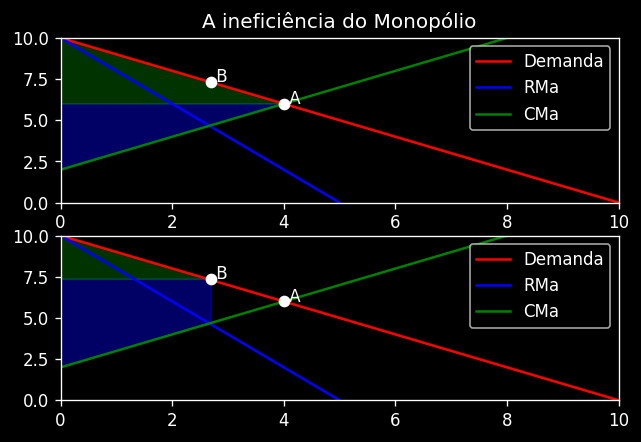
\includegraphics[scale=0.8]{cap25_4-inef_monopolio.png}
\end{center}

O gráfico da parte de cima é o equilíbrio no mercado de competição e o de baixo é o nosso equilíbrio com monopólio. Perceba como há um incremento no excedente do produtor (medido pela área azul) e uma redução do excedente do consumidor (área verde).
\\
\\
Para investigarmos se há uma ineficiência no sentido de Pareto no ponto $B$, façamos a seguinte pergunta: É possível adicionar uma unidade de produto no mercado de modo que o custo marginal pela produção desse bem seja inferior ao preço do mesmo? A resposta é claramente sim!
\\
\\
No nível $B$, a curva de preço (medida pela demanda inversa) ainda é superior à curva de custo marginal (aquela reta verde). Desse modo, se o monopolista produzisse mais uma unidade, ele receberia mais do que o custo marginal dessa unidade e os consumidores cujo preço de reserva é igual ao novo nível de preço passariam a consumir o produto. O excedente desse novo consumidor é igual a $0$, contudo, todos os que já consumiam o produto passaram a pagar menos do que antes o que aumentará os seus respectivos excedentes. Como o consumidor teria um lucro positivo (pois o custo marginal é inferior ao preço) e os consumidores teriam um aumento de excedente, achamos uma melhoria de Pareto.
\\
\\
A razão para o monopolista abrir mão dessa receita adicional é devida a necessidade dele de ter que manter o mesmo preço para todos os compradores\footnote{Vamos explorar mais essa ideia no próximo capítulo.}. Diferente da empresa na competição perfeita, ele leva em consideração o impacto dessa unidade adicional no lucro. Essa redução do lucro se dá porque ao produzir mais, o preço de todas as unidades cai. Se ele pudesse manter o preço nas unidades anteriores e vender mais barato as novas, ele venderia. 

\section{O Ônus do Monopólio}

Agora que já vimos que o monopólio é ineficiente, podemos querer mensurar o tamanho dessa ineficiência. Uma maneira possível de medir essa ineficiência é observando os excedentes nos cenários competitivo e de monopólio. Observe a figura abaixo:

\begin{center}
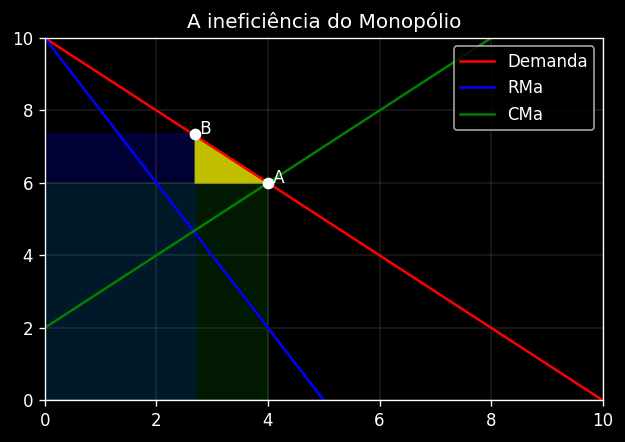
\includegraphics[scale=0.8]{cap25_5-onus_monopolio.png}
\end{center}

A área amarela é a medida da redução do excedente do consumidor. Em vermelho temos a redução do excedente do produtor. Em branco temos o quanto o monopolista consegue "capturar"\ do excedente dos consumidores ao adotar o nível de produção que maximiza o seu lucro.
\\
\\
A área branca não é definida como parte da ineficiência porque ela apenas demonstra uma transferência de excedente dos consumidores para o produtor. O \textbf{ônus resultante do monopólio} é precisamente a soma das áreas amarela e vermelha.
\\
\\
\textbf{Comentário:} Aqui o professor discorre sobre 3 exemplos do ônus do monopólio. Eu vou dar um resumo mas indico que você leia essa parte do livro.
\\
\\
No exemplo 1, vemos os casos das patentes (que, na prática, podem ser entendidas como um monopólio temporário). A ideia das patentes é criar um incentivo ao investimento em pesquisa e desenvolvimento de novas tecnologias. Contudo, por se tratar de um monopólio, acaba por criar um ônus atrelado a ele. O trabalho do Nobel William Nordhaus, demonstra que a estimativa da eficiência das patentes americanas é de 90\%, isso quer dizer que os consumidores estariam perdendo aproximadamente 10\% do seu excedente. O que parece indicar que o sistema de patentes não tem causado grandes malefícios.
\\
\\
No exemplo 2, ainda analisamos o mercado de patentes. Vemos que as patentes possuem 3 critérios de classificação: tempo de duração, extensão da proteção e novidade da invenção. Sendo os últimos dois muito subjetivos . Também discorremos sobre como o mercado de patentes permite algumas distorções (como o emaranhamento de patentes) de modo a tornar obrigatório para as empresas muito grandes a busca por grandes quantidades de patentes afim de se proteger de eventuais processos judiciais.
\\
\\
No exemplo 3, vemos o caso da isenção às proibições de \textit{antitrust} que os produtores agrícolas possuem nos EUA. Isso levou a uma pressão por parte dos grupos organizados dos produtores de batata a forçarem uma redução na quantidade ofertada do produto na ordem de 6,8 milhões de sacas. O que seria equivalente a 1,3 bilhão de pedidos de batata frita.

\section{Monopólio Natural}

Pois bem, já aprendemos o modelo de decisão do monopolista e também já vimos a ineficiência que esse modelo acarreta para os mercados. Ao percebemos que o monopólio produz aquém da quantidade ótima, poderíamos nos sentir tentados a propor regulações que obrigassem o monopolista a aumentar o seu nível de produção até o nível da competição perfeita. Contudo, esse problema é mais complexo do que parece, porque essa proposta de solução não leva em consideração a estrutura de custos.
\\
\\
Você mesmo pode fazer esse experimento, abra a simulação 25.2 ou a 25.3 e altere apenas o parâmetro "CF"\ que quer dizer "Custo Fixo". A medida que você aumenta esse parâmetro a curva de custo médio vai "subindo"\ e, em todos os pontos onde ele for superior a demanda, o monopolista terá lucro negativo.
\\
\\
Eu fiz 3 simulações para o caso da demanda com elasticidade constante. Uma com um custo fixo baixo, outra com um custo um pouco mais elevado e última com 10 vezes o custo fixo da primeira. Perceba ma imagem abaixo como a curva de lucro (da parte de baixo de cada painel vai caindo até desaparecer.

\begin{center}
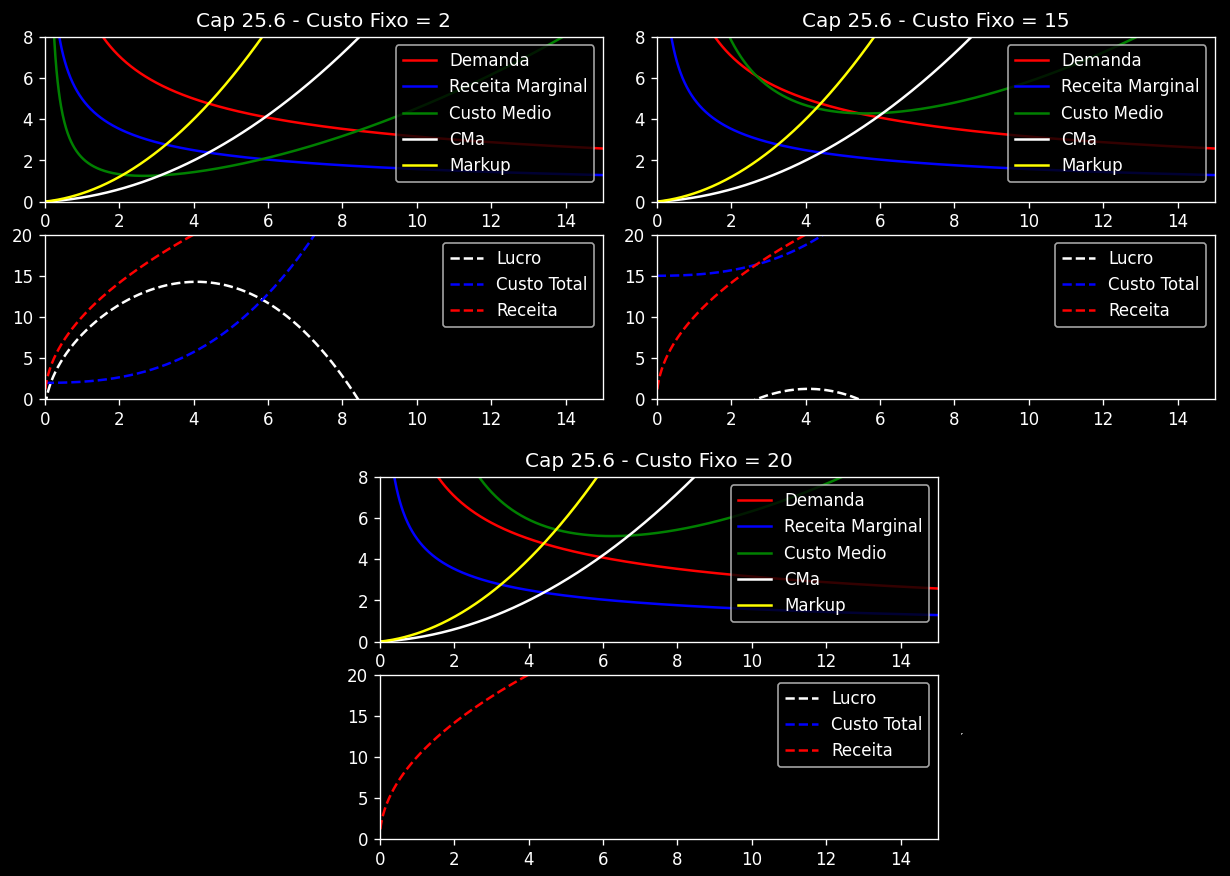
\includegraphics[scale=0.38]{cap25_6-monopolio_natural.png}
\end{center}

Chamamos de \textbf{monopólio natural} a situação onde temos uma estrutura de custo fixos fixos muito alta e custos marginais baixos. Agora podemos ver que se obrigarmos o monopolista a produzir o nível da competição perfeita, pode acontecer do projeto não ser sustentável, pois a curva de custo médio está acima da curva de demanda.
\\
\\
Agora o dilema ficou um pouco mais complexo. Se forçarmos o monopolista a produzir a quantidade que iguala o custo marginal ao preço, ele terá prejuízo. Se aceitarmos que ele mesmo defina a quantidade a produzir, agirá num ponto que produzirá uma ineficiência no mercado.
\\
\\
Não existe solução simples para essa questão. Na maioria das situações os monopólios naturais são regulamentados ou operados diretamente pelos governos. Cada opção de solução acaba acarretando benefícios e malefícios consigo. Em ambos os casos, os problemas são geralmente oriundos devido a informação assimétrica entre a empresa e os seus controladores.

\section{O Que Causa os Monopólios?}

Parabéns, querido aluno. Agora você já compreendeu como um monopolista age, o que o comportamento dele acarreta no mercado e como o controle sobre o monopólio é mais complexo do que se parece a primeira vista. Agora nos resta uma última investigação: Qual a causa dos monopólios?
\\
\\
Uma variável que podemos creditar como importante é a \textbf{escala mínima de eficiêntia (EME)}. Ela nada mais é do que o ponto de mínimo da nossa curva de custo médio.\footnote{Podemos achar esse ponto pela derivada primeira da função custo médio igual a zero e pela derivada segunda menor igual a zero.} O formato da curva de custo médio (e consequentemente a EME) é definido exclusivamente pela tecnologia.
\\
\\
Quando temos uma escala mínima de eficiência muito elevada, uma empresa precisa produzir uma quantidade muito grande dos bens vendidos no mercado para se manter. A economia é advinda da economia de escala. O que implica em uma capacidade produtiva de porte elevado. Nesses mercados, a chance maior é que hajam poucos ofertantes, e consequentemente, que esses ofertantes acabem usufruindo do poder de mercado advindo da pouca competitividade.
\\
\\
Quando temos uma EME pequena, qualquer empresa pequena pode começar a operar no mercado. Isso aumenta o número de competidores. O que acaba por reduzir o peso de cada empresa individualmente. O que acaba por gerar um ambiente de competição.
\\
\\
Observe que o fator importante é a relação entre a EME e o tamanho do mercado. É possível que a quantidade de eficiência aconteça em 10.000 de unidades, mas se o mercado for o Brasil inteiro, ainda pode ser que hajam muitos ofertantes. Quando não é possível aumentar o tamanho do mercado e a EME é elevada, aí sim, nos deparamos com uma condição de monopólio que pode necessitar de regulação ou mesmo intervenção do Estado.
\\
\\
Além da EME, outra maneira de se criar um monopólio é por meio da coordenação dos agentes ofertantes em uma \textbf{colusão}\footnote{Um ajuste secreto entre ofertantes para prejudicar outras pessoas.}. Quando um conjunto de empresa se une para definir em conjunto a produção, elas agem como um \textbf{cartel}. Esse cartel acaba atuando como se fosse um ofertante só (e consequentemente, age com o poder de mercado advindo dessa coordenação).
\\
\\
Um terceiro e último motivo para o nascimento de um monopólio é o bom e velho "cheguei primeiro". Se uma empresa, por algum acidente histórico, é a primeira a se estabelecer no mercado. É natural que ela se valha da falta de competidores e consiga um crescimento em escala. Quando novos ofertantes entram no mercado, o monopolista consegue usar seu arsenal de escala e reduzir artificialmente o preço até o ponto onde ninguém além dele pode se manter.
\\
\\
\textbf{Comentário:} Aqui o professor cita alguns exemplo. Mesma coisa de antes, indico ler o livro porque eu só vou dar uma resumida aqui.
\\
\\
No exemplo 1, vemos ocaso do mercado de diamantes e a sua gigante participante De Beers. É um exemplo de monopólio por tamanho da participação no mercado.
\\
\\
No exemplo 2, temos um caso de poder de mercado advindo da cooperação de comerciantes de móveis antigos.
\\
\\
No exemplo 3, outro exemplo de conluio por parte dos ofertantes para fixação dos preços de microchips de memória RAM.

%%%%%%%%%%%%%%%%%%%%%%%% CHAPTER %%%%%%%%%%%%%%%%%%%%%%%%
\chapter{O Comportamento do Monipolista}

\begin{chapquote}{The Godfather}
	``Great men are not born great, they grow great \dots''
\end{chapquote}

Na prática, a maioria das empresas possui algum poder de mercado. É bem possível que um mercadinho eleve um pouco seus preços sem que isso acarrete a perda de todos os seus clientes. Nesse capítulo vamos ver quais estratégias as empresas podem adotar para aumentar e explorar o seu poder de mercado.
\\
\\
A medida que você vai avançando no seu curso de Microeconomia, o seu arcabouço de conhecimento vai ficando cada vez mais refinado e, consequentemente, próximo da realidade. Os modelos puros de competição perfeita e monopólio até existem, mas são mais raros na realidade quando comparados à competição monopolística.\footnote{Veremos mais sobre isso nesse capítulo.}

\section{Tipos de discriminação de Preços}

No capítulo anterior, nós vimos que o monopolista acaba produzindo em um ponto onde a demanda ainda está disposta a pagar por mais do que o custo marginal. Vimos que a explicação do porquê ele não produz mais é que ele teria de baixar o preço de todos os produtos e não apenas os adicionais. Pois bem, existem alguns monopolistas que detém o poder de \textbf{discriminação de preços}. O professor classifica esse poder em 3 categorias:

\begin{itemize}
\item Discriminação de Preços de 1º Grau:
	\begin{itemize}
	\item[] Nesse caso ele tem poder de cobrar um preço diferente para cada consumidor e para cada quantidade.
	\end{itemize}
\item Discriminação de Preços de 2º Grau
	\begin{itemize}
	\item[] Nesse caso ele tem poder de discriminar o preço apenas para as quantidades compradas. Mas todos os consumidores que levarem a mesma quantidade, pagarão o mesmo preço no total.
	\end{itemize}
\item Discriminação de Preços de 3º Grau
	\begin{itemize}
	\item[] Esse é o caso mais comum. É quando o monopolista tem o poder de escolher qual preço cada pessoa vai pagar por todas as unidades que levar. Ou seja, ele pode controlar qual o valor de todas as unidades da cesta, contudo, não pode diferenciar o valor entre essas unidades.
	\end{itemize}
\end{itemize}

\section{Discriminação de Preços de 1º Grau}

Nesse caso, o monopolista está em \href{https://www.encurtador.com.br/eqCN1}{plenos poderes}. Ele possui conhecimento do preço de reserva\footnote{Lembra desse conceito?} de cada consumidor e, com esse conhecimento, cobra exatamente o valor máximo para cada quantidade. Também chamamos esse tipo de \textbf{discriminação perfeita}.
\\
\\
Um fato curioso desse arranjo é que, por incrível que pareça, ele é eficiente no sentido de Pareto. Uma vez que, para cada produto vendido, os consumidores pagam exatamente o valor máximo que estão dispostos a pagar, e consequentemente, o monopolista vai vender para todos os consumidores que tenham um preço de reserva maior ou igual ao custo marginal. O ponto final da produção será o ponto onde a quantidade iguala o custo marginal à curva de demanda.
\\
\\
Em termos de excedente, o que acontece é que o monopolista captura todo o excedente do mercado. Os consumidores, por sua vez, não possuem nenhum excedente.

\begin{figure}[H]
\centering
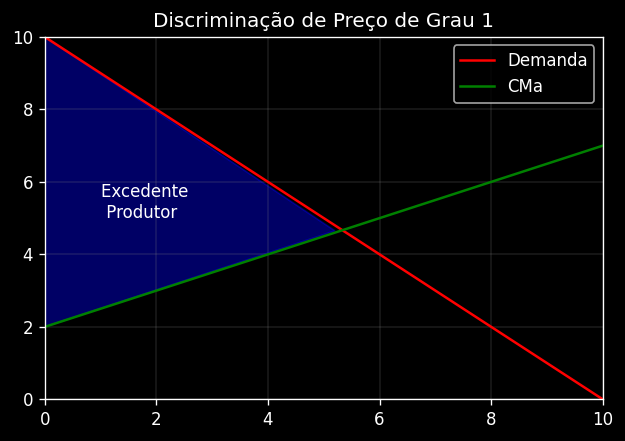
\includegraphics[scale=0.6]{cap26_2-discriminacao_grau1.png}
\end{figure}

Uma maneira conveniente se se pensar nessa situação é pela ótica da produção. Ao invés de pensar que o produtor olha para cada cliente e consegue cobrar exatamente o máximo que ele quer pagar, ele simplesmente oferta no mercado uma quantidade e deixa que os clientes definam quanto pagarão por ela. Claro que estamos supondo uma simplificação do comportamento das pessoas, mas a ilustração é válida.
\\
\\
O professor cita um exemplo da companhia aérea chamada Southwest Airlines. Que usou um software chamado Ding que faz ofertas periódicas e exclusivas para cada cliente cadastrado no sistema. Outro exemplo menos real, e mais icônico, é Mafioso Don Vito Corleone da clássica trilogia de filmes The Godfather (na abertura de todos os capítulos desse manual contém uma frase retirada dessa obra). O "modelo de negócio"\ do protagonista é fazer alguns favores em troca de outros favores. No caso do personagem mafioso, ele abusava do poder de mercado que detinha para cobrar o máximo possível (em bens ou serviços) de quem estava em dívida com ele.
\\
\ 
\\
\begin{figure}[H]
\centering
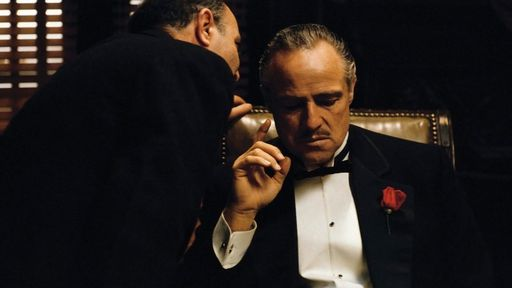
\includegraphics[scale=0.5]{cap26_2-don_corleone.jpeg}
\caption*{The Godfather (1972) - Paramount Films}
\end{figure}

\section{Discriminação de Preços de 2º Grau}

Nesse modelo, também chamado de \textbf{fixação de preços não linear}, o produtor já não pode cobrar, por uma mesma quantidade, um valor diferente entre consumidores diferentes. Isso força o monopolista a desenvolver uma estratégia de precificação que tente tirar o maior proveito possível das diferentes curvas de demanda.
\\
\\
\textbf{Comentário:} Eu não sei você, mas no meu caso, deu um trabalhão para entender o que o professor quis dizer nessa parte. Eu acho que o que deixou mais confuso foi ele ter suposto que o custo marginal é igual a zero (porque isso implicaria em dizer que ele venderia alguma cesta ao preço zero). Então eu retirei essa simplificação e reconstruí a mesma argumentação dele só que para um custo marginal constante maior que zero.\footnote{\href{https://www.youtube.com/watch?v=OBgziVdHH8w}{Esse vídeo aqui me ajudou bastante a entender melhor o que o professor quis dizer.}}
\\
\\
Imagine que temos apenas $2$ grupos de consumidores no mercado. Como nosso modelo prevê, o monopolista tem acesso as curvas de demanda de cada consumidor, mas como limitação, ele só pode escolher quais cestas ofertar por qual preço, e deixar que os consumidores escolham qual é a melhor para eles. Chamamos esse modelo de \textbf{autosseleção}.
\\
\\
O objetivo do monopolista é captar todo o excedente do mercado. Mas ele enfrenta uma limitação nessa modalidade de discriminação de preços. Como ele não pode vender a mesma quantidade a preços diferentes para os grupos de consumidores, ele tem de escolher se vai vender a preço de reserva da curva de demanda 1 ou 2.

\begin{figure}[H]
\centering
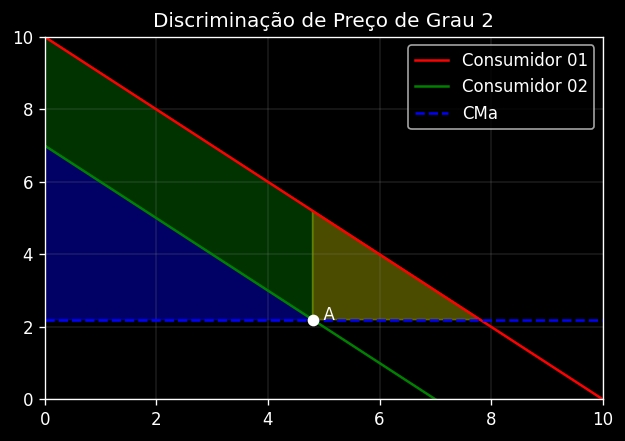
\includegraphics[scale=0.8]{cap26_3-discriminacao_grau2_1.png}
\end{figure}

Se ele optar por vender na fronteira da curva de demanda 1, ele vai abrir mão de todo o excedente advindo dos consumidores do tipo 2! Isso significaria abrir mão do toda a área azul na figura acima. Como ele não vai fazer isso, ele adotará a seguinte abordagem: Vender de $0$ até o ponto $A$ pelo preço de reserva da curva de demanda dos consumidores do tipo 2 e, a partir desse ponto, vender pela fronteira do preço de reserva dos consumidores do tipo 1. Isso garantirá que ele obtenha todo o excedente da área azul e também da área amarela.
\\
\\
Não satisfeito, o monopolista pode pensar um pouco mais e perceber que ele pode escolher uma opção que aumentará o seu excedente. Veja o que acontece se ele decide optar pela fronteira do consumidor tipo para uma cesta cuja quantidade é um pouco menor que a cesta $A$.

\begin{figure}[H]
\centering
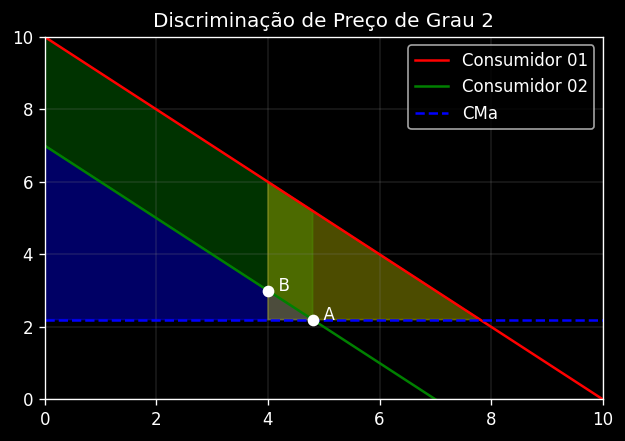
\includegraphics[scale=0.8]{cap26_3-discriminacao_grau2_2.png}
\end{figure}

Veja só que interessante, como no ponto $B$ o preço não é igual ao custo marginal para o consumidor tipo 2, haverá uma perda no total do excedente capturado pelo monopolista, mas em contrapartida, veja como a área amarela aumentou muito mais do que a área de perda do excedente do primeiro grupo. Isso quer dizer que, ao aumentar o preço da cesta, optando por adotar o preço de reserva do consumidor tipo 1 em um ponto anterior ao custo marginal igual à demanda tipo 2, o monopolista "abre mão"\ de uma pequena parte do excedente tipo 1 e ganha uma grande parte do excedente tipo 2. Não é difícil prever que ele continuará reduzindo a quantidade até o ponto onde o excedente perdido de um grupo é igual ao excedente ganho do outro.

\begin{figure}[H]
\centering
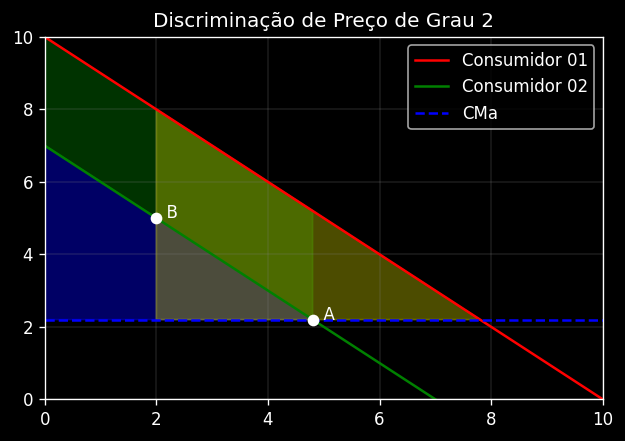
\includegraphics[scale=0.8]{cap26_3-discriminacao_grau2_3.png}
\end{figure}

A partir desse novo ponto $B$, o excedente perdido dos consumidores tipo 2 com o aumento do preço da cesta é maior que o ganho adicional do excedente dos consumidores tipo 1. Desse modo o monopolista acaba com um excedente total igual à área azul e toda a área amarela.
\\
\\
\textbf{Comentário:} Alguns de vocês podem pensar que o excedente abaixo da curva de demanda verde foi inteiramente perdido. Mas não é o caso! Perceba que, mesmo com a retirada dos consumidores do tipo $2$, essa área de excedente foi preenchida pelo excedente dos consumidores do tipo $1$. O monopolista abre mão no sentido que antes essa área era computada duas vezes (uma vez para cada tipo de consumidor).
\\
\\
Na realidade, o principal método de incentivo a autosseleção é a alteração da qualidade do bem. Normalmente, o monopolista reduz a qualidade dos produtos direcionados aos consumidores com preços de reserva menores, afim de eviter que seus consumidores dispostos a pagar mais, prefiram comprar esses produtos ao invés de produtos de "primeira linha". Essa estratégia maximiza o lucro do monopolista e ainda garante algum excedente para os consumidores das demandas mais altas.
\\
\\
O professor coloca dois exemplos que são espetaculares. Um sobre a diferença nos preços das passagens aéreas e o motivo da existência das classes econômica e executiva nos meios de transporte. Recomendo demais a leitura. O segundo é referente ao mercado de remédios.

\section{Discriminação de Preços de 3º Grau}

Só nos resta o último tipo de discriminação de preços. Nesse caso, o monopolista consegue discernir claramente qual consumidor pertence a qual grupo e, consequentemente, consegue cobrar um preço diferente. Atente para o fato que o monopolista só pode adota um único preço para cada grupo de consumidores.
\\
\\
Na prática, a modelagem desse problema é muito parecida com o que vimos no capítulo passado, já que, ele só pode escolher um único preço para cada tipo de consumidor. A única diferença do modelo do capítulo passado é que ele vai se deparar com mais de uma curva de demanda. Veja a formalização do problema logo abaixo

\begin{center}
\LARGE $\stackrel{máx}{\text{\small $y_1,y_2$}} \ \ \stackrel{p_1(y_1)y_1 + p_2(y_2)y_2 - c(y_1 + y_2)}{\ }$ \\
\end{center}

Esse problema nada mais é do que uma adaptação do problema da maximização da receita. Veja que $p_1(y_1)y_1$ nada mais é do que a receita obtida com a venda do produto para o grupo 1. Desse modo, o problema de maximização é a receita total obtida (que é a soma das receitas da venda para cada grupo) menos o custo total de produção.
\\
\\
Da mesma maneira de antes, a otimização será dada por:

$$ RM_1(y_1) = CMa(y_1+y_2) $$
$$ RM_2(y_2) = CMa(y_1+y_2) $$
Isso claramente implica em
$$ RM_1(y_1) = RM_2(y_2) = CMa(y_1+y_2) $$

\textbf{Atenção:} Eu acho que encontrei um erro de tradução no parágrafo que vem logo depois dessa expressão das receitas marginais acima. Na tradução, temos o trecho: "se a receita marginal no mercado 1 ultrapassar o custo marginal, valeria a pena aumentar a produção \textbf{nos dois mercados}". Isso está errado! No original temos a seguinte passagem: "if the marginal revenue in market 1 exceeded marginal cost, it would pay to expand output \textbf{in market 1}, and similarly for market 2". Uma tradução melhor seria algo como: "se a receita marginal no mercado 1 for maior que a o custo marginal, então valerá a pena aumentar a produção no mercado 1, a mesma lógica se aplica ao mercado 2".
\\
\\
Podemos usar a nossa fórmula da elasticidade para elaborar um pouco mais esse problema:

$$ p_1(y_1) \left[1 - \frac{1}{|\epsilon_1(y_1)|} \right] = CMa(y_1 + y_2) $$
$$ p_2(y_2) \left[1 - \frac{1}{|\epsilon_2(y_2)|} \right] = CMa(y_1 + y_2) $$
\\
Suponha que $y_1 = y_2$. Se $p_1 > p_2$, então:

$$ 1 - \frac{1}{|\epsilon_1(y_1)|} < 1 - \frac{1}{|\epsilon_2(y_2)|} $$
\\
O que implica em

$$ \frac{1}{|\epsilon_1(y_1)|} > \frac{1}{|\epsilon_2(y_2)|} $$
\\
Que, por fim, nos diz que

$$ |\epsilon_1(y_1)| < |\epsilon_2(y_2)| $$
\\
Não continue lendo se você não entendeu essa afirmação. Pare e pense até sentir que compreendeu o argumento. Se ainda tiver dúvida \href{https://twitter.com/bruno_ruas2}{me manda um twite que eu te ajudo}.
\\
\\
Dessa maneira, podemos ver que quanto mais elástico for o mercado, menor será o seu preço. Faz todo sentido porquê quanto mais elástica é a demanda, mais sensível ela será às alterações de preços. Portanto, o monopolista vai conseguir elevar o preço sempre que a demanda for inelástica e manterá o preço comparativamente mais baixo nos grupos de demanda mais elástica. Isso maximizará o seu lucro em cada grupo de consumidores.
\\
\\
\textbf{Comentário:} Querido aluno, agora você tem todo o arcabouço teórico necessário para entender o motivo de você pagar meia entrada no cinema\footnote{Entender isso é muito top, fala sério.}. Os cinemas acreditam que uma elevação dos preços levaria vocês a buscar outros serviços além do cinema, visto que é comum supor que essa fase da vida tenha restrição orçamentária consideravelmente modesta. Por outro lado, um executivo de uma empresa tem um preço de reserva muito maior que o de vocês, então o cinema cobra dele mais caro para entrar (sem falar o preço "salgado"\ das pipocas).
\\
\\
Agora o professor coloca três exemplos. O primeiro é teórico, o segundo é um exemplo de aplicação e o terceiro é uma aplicação do conceito ao mercado de revistas acadêmicas. Eu vou criar uma simulação do segundo exemplo.

\subsection{Curvas de Demanda Lineares}

O monopolista precisa lidar com duas curvas de demanda (que suporemos serem lineares) do tipo:

$$ D_1(p_1) = 100 - p_1 $$
$$ D_2(p_2) = 100 - 2p_2 $$
\\
As demandas inversas dessas funções são

$$ p_1(y_1) = 100 - y_1 $$
$$ p_2(y_2) = 50 - y_2/2 $$
\\
As funções de receita serão iguais a

$$ r_1(y_1) = 100y_1 - y_{1}^{2} $$
$$ r_2(y_2) = 50y_2 - \frac{y_{2}^{2}}{2} $$
\\
Cujas receitas marginais serão

$$ RMa_1(y_1) = 100 - 2y_{1} $$
$$ RMa_2(y_2) = 50 - y_{2} $$
\\
Para simplificar vamos supor que o custo marginal é contante em $CMa = \$ 20,00 $. Com isso já podemos criar uma simulação do modelo. Mas antes de colocar o computador fazer isso, nós podemos encontrar os pontos de máximo facilmente ao igualar as funções de receita marginal ao custo marginal.

$$ 100 - 2y_{1} = 20 \hspace{100pt} 50 - y_{2} = 20 $$
$$ 100 - 20 = 2y_{1} \hspace{100pt} 50 - 20 = y_{2} $$
$$ 80/2 = y_{1} = 40 \hspace{120pt} y_2 = 30 $$
\\
Sabemos que os pontos de maximização do lucro para cada curva de demanda serão os pontos cujas quantidades são iguais a $y_1 = 40$ e $y_2 = 30$. Para descobrir os preços, basta colocar esses valores nas funções de demanda inversa. Podemos ver que esses são os pontos que estão no topo das curvas de lucro 1 e 2.

\begin{figure}[H]
\centering
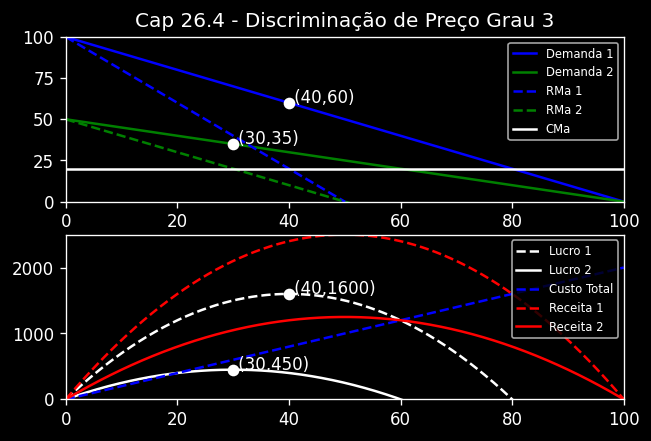
\includegraphics[scale=0.8]{cap26_4-discriminacao_grau3.png}
\end{figure}

\textbf{Simulação:} \href{https://colab.research.google.com/drive/1TYSpJLSEg4yInKX_viA6aP8qLiRsHdBm?usp=sharing}{Clique aqui} para ter acesso a essa simulação.
\\
\\
Se, por outro lado, o monopolista não puder fazer essa separação dos preços, teremos que somar as demandas como se fosse uma única e trabalhar a otimização como no primeiro modelo do capítulo 25.

\begin{figure}[H]
\centering
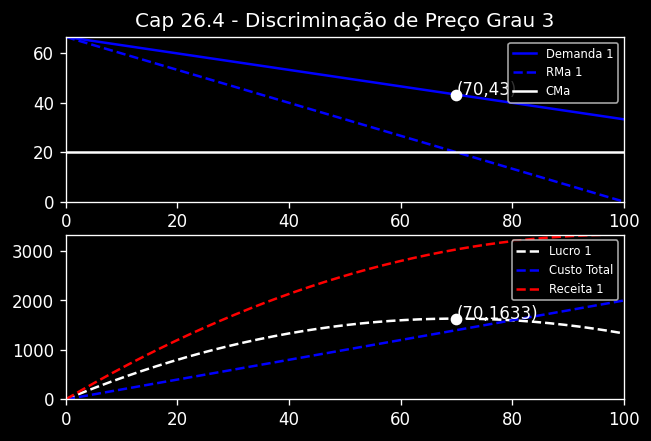
\includegraphics[scale=0.8]{cap26_4-discriminacao_grau3_2.png}
\end{figure}

\textbf{Atenção:} Quando trabalharmos com demandas somadas, temos que testar se o preço de equilíbrio não gera demanda negativa em alguma das curvas de demanda. Se a função demanda for negativa ao preço de equilíbrio, isso quer dizer que o monopolista aumentará o seu lucro se não vender para esse grupo de consumidores. Ao excluir essa demanda e calcular o novo equilíbrio, seu lucro aumentará.

\section{Vinculação de Produtos}

Uma prática muito comum entre as empresas é a \textbf{venda casada}. Você já se perguntou qual o motivo das empresas de internet se esforçarem tanto para vender o pacote TV + Internet + Telefone?. Pois bem, agora você vai ter uma ideia por trás dessa estratégia.\footnote{Aqui estamos supondo que as demandas por esses serviços não são relacionadas. Mas não leve esse primeiro parágrafo tão ao pé da letra. O objetivo dele é só vender o conteúdo do tópico ;)}
\\
\\
Já vimos que a vontade do monopolista é cobrar o máximo possível para cada cliente em cada quantidade. Isso faria com que ele capturasse todo o excedente do mercado. Como na prática isso implicaria em conhecimento perfeito de todos os consumidores e existe uma legislação que limita a capacidade de impor muito do poder de mercado, as empresas se valem de estratégias para maximizar esse excedente.
\\
\\
Uma dessas estratégias é exatamente a venda casada. A ideia é a seguinte: como o vendedor não pode cobrar um preço para cada consumidor, ele precisa ter uma ideia dos preços de reserva dos mesmos para que possa cobrar exatamente o valor do preço de reserva mais baixo que o custo marginal permita.
\\
\\
Veja a tabela 26.1 a página 672 do livro. Temos dois tipos consumidores que possuem preços de reservas inversos para dois tipos de programas diferentes. Se o monopolista cobrar $U\$ 101,00$ pelo processador de texto, ele perderá 100\% dos consumidores do tipo A. Por causa disso, ele sempre cobrará o mínimo possível para poder capturar o preço de reserva mais baixo. Isso implica que os consumidores que possuem preços de reserva maiores tenham algum excedente.
\\
\\
Mas como bem sabemos, as empresas sempre pensam em novas estratégias. No caso da vinculação de produtos, supondo que o preço de reserva pelos produtos juntos seja igual à soma dos preços individuais, nós tratamos os dois produtos como uma cesta única. Nesse novo arranjo, o vendedor consegue cobrar um preço maior, porque o preço de reserva por cesta é maior que o valor cobrado separadamente.
\\
\\
Eu expandi um pouco do exemplo do professor Varian para um caso de 1.000 consumidores. Nessa simulação os preços de reserva são aleatórios entre 51 e 100. Para cada uma das duas abordagens, eu comparei os lucros a medida que se eleva o preço praticado no mercado. Para efeito de simplificação, os preços de reserva mínimos são iguais nos dois produtos, então o vendedor sempre aumentará os preços em paralelo. Atente para o fato de que nesse gráfico o preço está no eixo horizontal.\footnote{Ficou na dúvida, fala comigo que eu explico melhor.}

\begin{figure}[H]
\centering
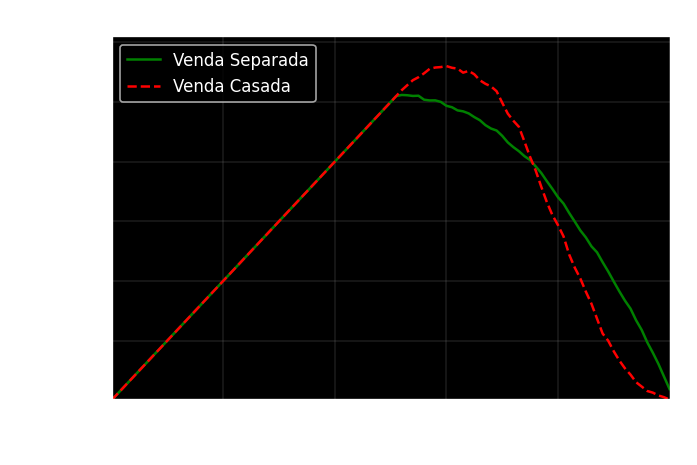
\includegraphics[scale=0.8]{cap26_5-venda_casada.png}
\end{figure}

\textbf{Simulação:} \href{https://drive.google.com/file/d/1WhxGaAhUB9dKkgrKWadihIrzS4cm3bXP/view?usp=sharing}{Clique aqui} para ter acesso a essa simulação.
\\
\\
De zero até 50, a curva de lucro é uma linha reta porque o preço de reserva mínimo da nossa simulação é 50. Então, sempre existirá alguém disposto a comprar a medida que ofertamos até esse preço. A partir desse ponto, cobrar mais caro implica em abrir mão dos consumidores com preço de reserva menor que o preço.

\section{Tarifas Bipartidas}

Um artigo famoso de 1971 cujo título é "A Disneyland Dilemma: Two-Part Tariffs for a Mickey Mouse Monopoly", de Walter Oi, nos mostra uma situação interessante. Como o monopolista se comportará no caso da venda de dois produtos que possuem demandas interrelaciandas?
\\
\\
No tópico anterior, supomos que as demandas eram independentes. Agora temos um caso onde, ao aumentar a oferta do bem 1, os consumidores estarão menos propensos a consumir o bem 2. Chamamos esse arranjo de \textbf{tarifa bipartida}.
\\
\\
Como já trabalhamos antes, sabemos que a maximização do lucro é obtida no ponto onde o custo marginal é igual à receita marginal. Fazendo isso para a oferta do bem 1 e como ele não pode discriminar perfeitamente os preços, haverá um excedente do consumidor. Esse excedente é exatamente o valor máximo que ele pode cobrar pelo bem 2. Nesse caso, pode ser que a quantidade cobrada pelo bem 2 seja inferior ao montante que iguale o custo marginal à receita marginal.
\\
\\
Para elucidar esse modelo eu fiz uma simulação. Fora suposto que as demandas são lineares, com a mesma forma funcional e interdependentes, ou seja, quanto mais de um bem se tem, menos do outro terá. Os custo marginais são fixos em 20.
\\
\\
Como esse problema envolve o equilíbrio em dois mercados (bem 1 e bem 2), eu optei por construir um gráfico tridimensional. O problema dessa abordagem é que a melhor maneira de se entender um gráfico desse é pela mudança do ângulo da câmera. Então eu vou colocar 3 perfis de visualização mas também fiz um gif com um panorama dos eixos \href{https://github.com/brunoruas2/Meus_Estudos/blob/main/Microeconomia/Microeconomics\%20-\%20Hal\%20Varian/images/cap26_6-tarifas_bipartidas.gif}{\textbf{clique aqui para ver}}.

\begin{figure}[H]
\centering
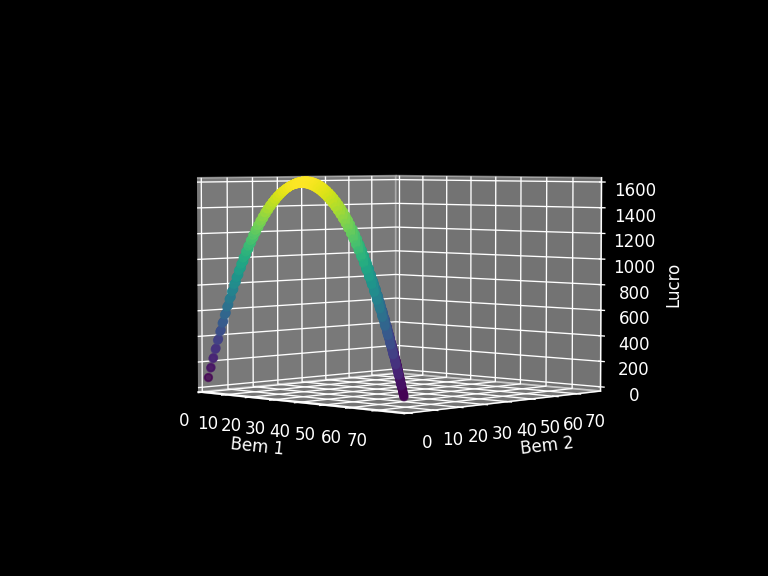
\includegraphics[scale=0.6]{cap26_6-tarifas_bipartidas1.png}
\end{figure}

Nessa primeira imagem temos um ângulo que evidencia como o lucro se comportaria se só existisse o mercado do bem 1. Podemos ver que o lucro é maximizado em um ponto (que é justamente onde o custo marginal é igual à receita marginal. A segunda imagem é similar a primeira, mas para o outro bem.

\begin{figure}[H]
\centering
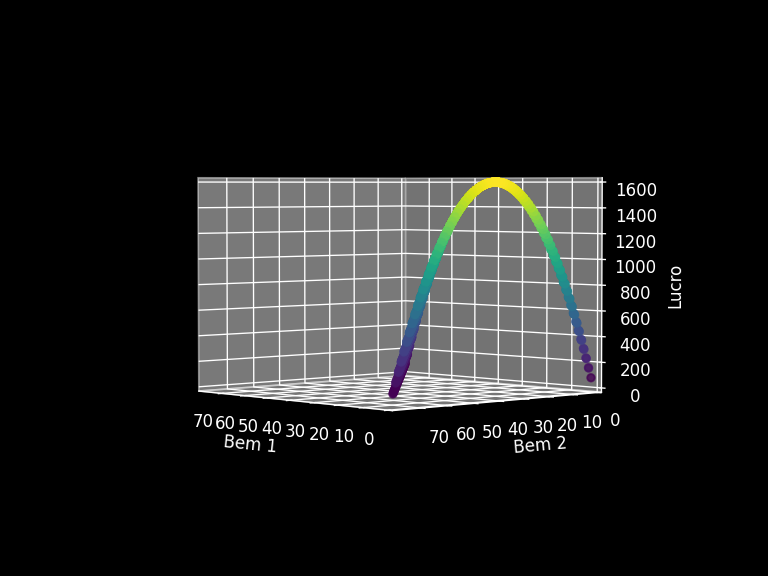
\includegraphics[scale=0.6]{cap26_6-tarifas_bipartidas2.png}
\end{figure}

A terceira mostra como o monopolista deverá agir para poder ofertar ambos os bens. O padrão é simétrico porque no modelo as duas demandas possuem as mesmas formas e os mesmos coeficientes. Veja como a figura do lucro forma um tipo de "onda"\ que parte da cesta onde os dois bens são iguais a zero. Na parte amarela temos o máximo do lucro possível para cada cesta. E, a partir desses pontos de máximo, os lucros de cada cesta vão sendo cada vez menores.

\begin{figure}[H]
\centering
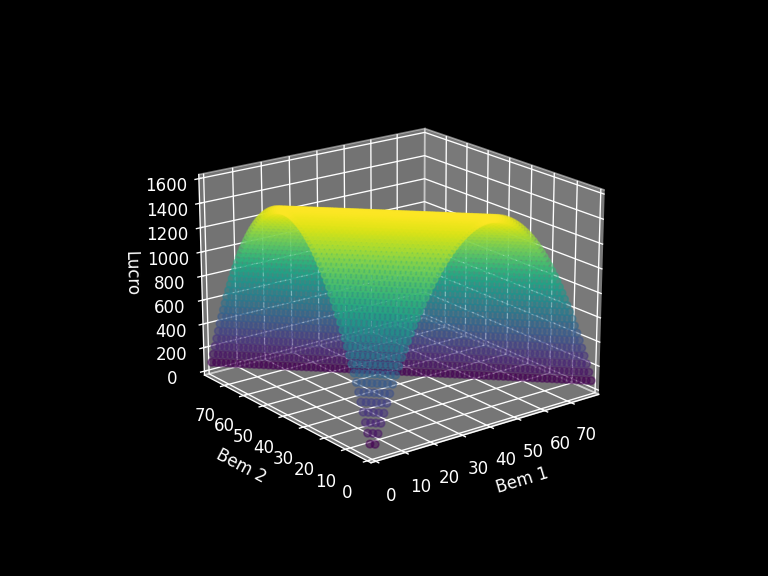
\includegraphics[scale=0.8]{cap26_6-tarifas_bipartidas3.png}
\end{figure}

A última mostra um ângulo onde vemos a relação de troca entre os bens (a linha vermelha indica a reta onde as cestas maximizam o lucro). Observe que, visto de cima, temos um gráfico que demonstra o quanto o monopolista tem que abrir mão de um bem para vender mais do outro, sem que isso incorra em redução do seu lucro total.\footnote{Pra mim, lembra um pouco a curva de restrição orçamentária do consumidor.}

\begin{figure}[H]
\centering
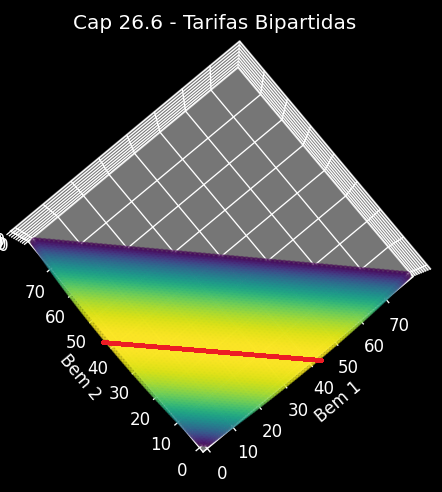
\includegraphics[scale=0.60]{cap26_6-tarifas_bipartidas4.png}
\end{figure}

Como as demandas desse modelo são simétricas e os custos são iguais, o modelo gráfico é uniforme. Na imagem abaixo eu simulei o mesmo modelo para o caso onde o custo marginal do bem 2 é igual a zero.

\begin{figure}[H]
\centering
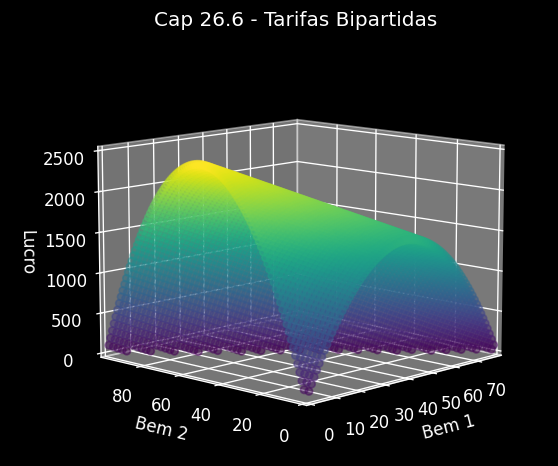
\includegraphics[scale=0.75]{cap26_6-tarifas_bipartidas5.png}
\end{figure}

Podemos ver claramente que, nesse segundo caso, o monopolista só maximiza seu lucro ao vender exclusivamente o bem 2.
\\
\\
Essa assimetria é a explicação do motivo da Disney não cobrar um preço pela entrada nos brinquedos, uma vez que em os custos dos serviços (a saber: a entrada e os passeios) não são iguais. A Disney percebeu que ao cobrar somente a entrada, poderia captar mais o excedente total do mercado do que se cobrasse também os passeios aos brinquedos.

\section{Competição Monopolística}

Nós começamos essa seção do livro partindo da posição oposta aos modelos que vimos ao longo da primeira metade do curso. Adaptamos o modelo da escolha maximizadora do lucro para a existência do poder de mercado e avançamos como o monopolista pode usar esse poder mesmo em arranjos menos favoráveis à capacidade de discriminação de preços. Nessas últimas duas seções expandimos nosso modelo para mais de um produto e como eles podem interagir entre si para a maximização do lucro.
\\
\\
Todo esse caminho foi muito bem pensado pelo professor. Lá no começo alguns de vocês podem ter achado a hipótese da existência de apenas um produtor um tanto quanto caricata. Mas agora vamos trazer o nosso modelo da escolha para mais perto da realidade presenciada todos os dias por vocês.
\\
\\
Até agora, tratamos uma \textbf{indústria} como um conjunto de produtores cujo resultado do esforço produtivo era \textit{exatamente} a mesma mercadoria. Isso quer dizer que, sendo 1 (que é o caso do monopólio) ou 1.000 produtores, todas as mercadorias que saem das fábricas e são comercializadas seriam exatamente as mesmas. Essa hipótese simplificadora vai dar lugar a uma nova que, na minha opinião, é bem mais aplicável a nossa realidade fática.
\\
\\
Os produtos agora possuem certas propriedades exclusivas (sendo a marca a principal) e seus competidores também serão diferenciáveis entre si. Todos competindo por um mercado de bens relativamente parecidos aos consumidores. Além disso, vamos considerar que a barreira de entrada de novos produtores também será mais baixa.
\\
\\
Nesse novo arranjo, os produtores possuem características de ambos os modelos vistos. Eles não podem alterar seus preços completamente como um monopólio, porque os consumidores olhariam para os seus concorrentes e comprariam algum produto semelhante ao seu, só que mais barato. Por outro lado, eles não estão fadados estritamente ao preço de mercado, uma vez que nesse arranjo a demanda não será infinitamente elástica. O nome dessa estrutura setorial é \textbf{concorrência monopolística}.\footnote{Eu não sei você, mas eu acho esse modelo muito empolgante de ser estudado.}
\\
\\
Estamos vendo apenas vantagens ao novo modelo, mas como tudo na vida, temos um trade-off entre realidade e praticidade. Esse modelo é bem mais complexo de ser construído e analisado. Como o próprio professor diz "Em um modelo detalhado do setor de competição monopolística, dependemos muito dos detalhes específicos dos produtos e da tecnologia (de produção), assim como da natureza das escolhas estratégicas disponíveis para as empresas". Isso acaba implicando naquela situação clássica de "cada caso é um caso". Por causa disso, e do fato desse curso ser introdutório, vamos apenas ver alguma das principais estratégias dos economistas para modelar esses mercados.
\\
\\
Mesmo sendo um modelo mais complexo, podemos evidenciar algumas características que independam de quaisquer fatores relacionados ao mercados específicos. O primeiro deles é relacionado ao número de competidores.
\\
\\
É razoável supor que se o número de concorrentes aumentar (algo que está muito relacionado às barreiras de entrada) haverá impactos na curva de demanda que a empresa está imposta. O primeiro impacto que podemos supor é que essa curva irá se aproximar mais da origem do plano cartesiano\footnote{Ou seja, ele vai acabar tendo que baixar mais o seu preço se quiser continuar vendendo a mesma quantidade.}. O segundo impacto previsto é que a elasticidade de demanda aumentara\footnote{Porque agora os consumidores podem escolher mais opções em relação a antes.}.
\\
\\
Se todas as empresas do mercado tiverem como objetivo o lucro. Quaisquer equilíbrio alcançado terá que obedecer algumas restrições:
\begin{itemize}
\item Cada empresa venderá o máximo possível. Ou seja, elas sempre optam por ofertar cestas que estejam na curva de demanda e não abaixo dela.
\item Cada empresa precisará maximizar seu lucro levando em consideração as imposições oriundas à sua curva de demanda da empresa.
\item Quanto mais competidores o mercado tiver, mais próximo de zero será o lucro das empresas contidas no mercado.
\end{itemize}

Do fato 1, podemos derivar o fato que quaisquer opções de maximização estão na própria curva de demanda\footnote{Afinal, ela mostra as maiores quantidades para cada nível de preço.}. Do fato 3, podemos ver que a medida que o número de competidores tende ao infinito, a cesta escolhida deve ser num ponto onde a curva de custo médio tangencia a curva de demanda\footnote{A lógica é que se $p > c(y)/y$ então $py - c(y) > 0$, o que contraria nosso postulado. Agora, se $p = c(y)/y$ então, $py - c(y) = 0$, que é exatamente o que estamos dizendo.}. Por fim, o nosso postulado 2 afirma que a maximização ocorrerá na curva de demanda, isso implica no fato que a curva de custo médio não cruzará a curva de demanda, porque se isso acontecer, as empresas terão lucro positivos.
\\
\\
Existem algumas características desse equilíbrio competitivo monopolizador:
\begin{itemize}
\item Ele é ineficiente no sentido de Pareto, porque a maximização ocorre pelo custo médio e não pelo custo marginal. Mesmo sendo uma situação de lucro zero, quando tratamos de eficiência, estamos trabalhando com a maximização do excedente do mercado. E isso se dá pelo custo marginal.
\item As empresa acabam por atuar num ponto a esquerda do nível de produção. Isso quer dizer que os consumidores acabam não tendo acesso a todas as mercadores que os produtores realmente poderiam lançar no mercado.
\end{itemize}

Um fato interessante desse segundo ponto é que temos um trade-off interessante. Vimos que as empresas até teriam como ofertar quantidades maiores, mas como a maximização do lucro se dá pelo custo médio, elas não produzem tudo que podem. Se quiséssemos aumentar a oferta dos produtos, teríamos que reduzir a quantidade de ofertantes. Isso realmente aumentaria a quantidade ofertada por cada empresa, mas em contrapartida, os consumidores teriam menos opções para escolher!. Esse é o tipo de situação onde não existe regra de ouro e cada caso é único.

\section{Modelo de Diferenciação de Produtos por Local (Estabilidade na Competição)}

Esse seção é inspirada no clássico artigo de 1929 "Stability in Competition"\ de Harold Hotelling.\footnote{Imagina como deve ter sido doido publicar um artigo em 1929.}
\\
\\
Como foi dito antes, as abordagens puramente teóricas nessa parte da teoria microeconômica são limitadas porque agora os aspectos únicos de cada mercado acabam tornando praticamente impossível deduzirmos leis gerais. Na seção passada nós já aprendemos como um concorrente monopolista possui algumas restrições e alguma liberdade advinda da diferenciação dos produtos (que não é absoluta, mas existe). Agora, porém, vamos abordar outro tipo de diferenciação: A geográfica.
\\
\\
Nossos modelos sempre adotaram que os consumidores não possuíam nenhum custo pela aquisição além do preço. Mas, na realidade, todos nós precisamos sair de casa e perdermos um tempo indo até o local onde teremos acesso aos produtos que desejamos\footnote{Ou optamos por pagar a bendita taxa de entrega do Ifood afim de termos a comodidade de receber a comida na porta de casa.}.
\\
\\
Pensando nisso vamos criar um \href{https://en.wikipedia.org/wiki/Thought_experiment}{experimento mental}:
\\
Imagine que a orla da Ponta Negra seja retilínea e que só seja permitida a venda de sorvetes mediante autorização da Prefeitura. Adicionaremos a restrição que a probabilidade de você encontrar um transeunte com calor é uniforme em toda a extensão da orla. Suporemos também que os preços dos sorvetes sempre serão iguais, que não há diferença de qualidade e que por motivos climáticos só exista um único sabor disponível.
\\
\\
Diante das características do mercado acima, onde o primeiro sorveteiro com licença da prefeitura deve instalar sua barraquinha?. Não é difícil chegar na conclusão que ele deve se instalar exatamente no meio da orla. Desse modo, a distância máxima que um transeuntes com calor terá de caminhar para aliviar seu desconforto térmico é de meia orla.
\\
\\
Agora vamos complicar um pouco mais. Supondo que outro sorveteiro consiga sua licença para vender na orla. Qual será o melhor arranjo?. Se usarmos o mesmo pensamento de antes, podemos supor que cada vendedor fique no ponto que corresponda a 1/4 e 3/4 do tamanho da orla. Nesse caso, todos os consumidores das áreas 1/4 e 2/4 estariam próximos ao vendedor 1. E os consumidores dos setores 3/4 e 4/4 estariam mais próximos do sorveteiro 2. No final teremos uma distância máxima de 1/4 da orla para cada consumidor e 1/2 da receita total para cada sorveteiro.
\\
\\
Tudo certo então? Terminamos?. Evidente que não. Ainda precisamos pensar no que cada vendedor fará. Como eles querem maximizar sua receita, cada vendedor terá o incentivo à se mover um pouco para o centro, porque desse modo ele manterá a sua demanda cativa e ainda "roubará"\ parte da demanda do seu colega de ofício. No final, ambos se encontrarão no centro da orla. Esse novo arranjo aumenta a distância máxima dos consumidores para 1/2 e mantém a receita dos sorveteiros em 1/2.
\\
\\
Esse é um exemplo de como a competição pelos clientes gerou um padrão menos eficiente na localização dos sorveteiros. Quanto menos agentes temos nos mercado, mais precisaremos nos preocupar com as estratégias que cada um deles adotará.\footnote{Se você começou a pensar em teoria do jogos, é isso mesmo!}
\\
\\
Como o próprio Hotelling pontua na página 53: "A importância e variedade das tendências aglomerativas\footnote{Ele está falando da tendência à convergência.} se torna evidente quando nos lembramos que a distância, usada nessa ilustração, é apenas um termo figurativo para uma grande convergência de qualidade". O que o autor quer dizer, é que ele usou essa analogia das distâncias apenas como uma ilustração. Mas ao invés dos vendedores possuírem uma commoditie separada geograficamente, podemos considerar vendedores um do lado do outro, mas com produtos um pouco diferentes. Pelo modelo de Hotelling, eles terão um incentivo à padronização dos seus produtos.
\\
\\
No Youtube, parece que os vídeos estão cada vez mais parecidos. Na música, observamos padrões de ritmo, temática e estrutura de tempos em tempos. Os filmes de super-heróis viraram uma moda que já dura uma década. Enfim, esse padrão de convergência é explicado relativamente bem pelos conceitos que desenvolvemos até agora. Esse modelo de convergência na competição continua muito poderoso desde sua descoberta em 1929. Agora você tem um ferramental novo para impressionar seus parentes nas reuniões de família. Use esse poder com moderação.

\section{Diferenciação de Produtos}

Uma característica muito interessante da ciência é que ela não se limita em continuar revisando seus conhecimentos. Embora o modelo do Hotelling tenha sido muito famoso, os cientistas continuaram fazendo pesquisas e construindo modelos que explicassem os fenômenos observados na realidade. \\
\\
Existem situações onde os produtores optam por buscar o oposto do modelo de convergência, eles investem na diferenciação dos seus produtos. Qual o sentido disso? nós já vimos que, quanto maior é o grau de diferenciação do produto, mais característica de monopólio o competidor terá. Então as empresas investem pesado em marketing para alterar a percepção dos consumidores e construir a ideia de uma marca "única". A Apple tem uma estratégia excelente nessa linha, para citar um exemplo.
\\
\\
Infelizmente, o livro não adentra muito além da demonstração que existe essa vertente de possibilidade dos mercados. O importante aqui é saber que a competição monopolística pode gerar tanto uma padronização dos produtos quanto uma excessiva diferenciação deles.

\section{Mais Sorveteiros}

Se a gente retomar o nosso experimento mental da orla da Ponta Negra. Alguns de vocês podem pensar: "Mas perai, e se colocarmos mais sorveteiros no mercado?". Pois bem, vamos ver o que acontece nessa situação.
\\
\\
Coloque um novo sorveteiro em qualquer lugar. Acontecerá que alguém vai ficar no meio. Os que estão nas proximidades, vão ter o incentivo de irem cada vez mais para perto do que está no meio, uma vez que eles mantém seus clientes a ainda "roubam"\ parte dos clientes do pobre sorveteiro do meio. Só que o sorveteiro do meio também é esperto. Se um dos dois das extremidades chegar perto demais, ele pode simplesmente ir para no sentido da extremidade. Ao passar pelo sorveteiro que veio de lá, ele captaria toda a receita da extremidade até a sua atual posição.
\\
\\
Mas quando o sorveteiro do meio passa a ser um sorveteiro da extremidade, o novo sorveteiro do meio terá o mesmo incentivo que ele teve e também irá de encontro a algum deles para trocar de lugar. O que podemos ver é que esse arranjo é dinâmico. Sempre existirá um incentivo de algum dos sorveteiros de mudar de posição. Mas não se desespere. A medida que temos mais e mais competidores, o padrão de convergência volta a aparecer.
\\
\\
\textbf{Comentário:} Embora eu tenha dito o padrão de aglomeração reapareça para quatro ou mais vendedores, eu só refiz a mesma afirmação que o professor fez no seu livro. Eu não sei você, mas eu não gosto muito de afirmações sem as devidas comprovações. Quando tiver mais tempo, eu atualizo essa seção com a demonstração que esse padrão realmente aparece para 4 ou mais vendedores.\footnote{Favorita meu repositório no Github para não parder as atualizações no material.}

%%%%%%%%%%%%%%%%%%%%%%%% CHAPTER %%%%%%%%%%%%%%%%%%%%%%%%
\chapter{O Mercado de Fatores}

\begin{chapquote}{The Godfather}
	``Give him a living, but never discuss the family business with him.''
\end{chapquote}

Quando falamos de produção, o mercado de fatores é muito relevante e até o momento não tocamos nesse assunto desde do capítulo 20. Agora que temos um \textit{framework} mais interessante como o comportamento do monopolísta, podemos pensar nas implicações para o mercado de fatores. Veremos algumas situações: 
\begin{enumerate}

\item Qual a diferença entre a demanda por fatores de um monopólio e de uma empresa competitiva.

\item O que acontece quando temos um mercado de fatores competitivo mas apenas um comprador\footnote{O nome desse arranjo é \textbf{monopsônio}. Pense nele como um monopólio do mundo invertido de stranger things.}.

\item Como será o arranjo onde há um monopolista no mercado de fatores e um monopolista no mercado de produto.

\end{enumerate}

\section{O Monopólio no Mercado do Produto}

Pensemos novamente na empresa que demanda fatores de produção. Sua demanda maximizadora será dada pelo ponto onde o custo marginal pela compra do fator é igual à receita marginal advinda do emprego desse fator. Supondo uma empresa que só possua um único fator de produção. Sua função de produção será dada por $y = f(x)$. A receita será dada pelo volume de produção e da demanda inversa do mercado, algo como, $R(y) = p(y)y$. 
\\
\\
O \textbf{Produto Marginal} de um fator de produção é obtido pela variação da função produção em relação à variação do fator observado. No nosso exemplo, só temos um único fator, então:

$$ PM_x = \frac{\delta y}{\delta x} = f'(x) $$
\\
Se você sobreviveu até aqui, deve estar entendo tudo tranquilamente\footnote{Parabéns! Você está cada vez mais perto de ler um paper e de expressar modelos como os economistas fazem.}. 
\\
\\
Como não é novidade, esse incremento marginal na produção será vendido e produzirá uma \textbf{Receita Marginal}. Podemos expor esse efeito pela expressão da  variação infinitesimal da receita dividida pela variação infinitesimal do produto.\footnote{O primeiro capítulo desse material é exatamente para você saber o que estamos fazendo aqui.}

$$ RM_y = \frac{\delta R}{\delta y} = p(y) + p'(y)y $$
\\
Até agora já vimos o impacto que um fator causa no produto e, do outro lado, o impacto que um produto causa na receita. Agora nos resta fazer a relação direta entre essas duas lógicas. Uma vez que $y = f(x)$, então, $p(y) = p(f(x))$. Podemos reescrever nossa equação da receita como:

$$ R(x) = p(f(x))f(x) $$

Agora que temos nossa função de receita explicitamente relacionada ao nosso fator de produção, podemos obter a relação chamada de \textbf{Produto da Receita Marginal} que mede o impacto na receita dada uma variação no fator de produção. Para obter-la usamos a derivada de $R(x)$ em relação à $x$. 
\\
\\
Mas essa derivada tem um pequeno toque de sofisticação adicional: temos que aplicar, ao mesmo tempo, a regra da multiplicação junto à regra da cadeia.\footnote{A regra da cadeia para $p(y) = p(f(x))$ nos diz que $\frac{d p(y) }{d x} = \frac{d p(y)}{d y} \frac{d y}{d x} $.}

$$ PRM_x = \frac{d R(x)}{d x} = p(y)f'(x) + f(x)p'(y)f'(x) $$
$$ = [p(y) + p'(y)y]f'(x) $$
$$ = RM_y \times PM_x $$
\\
Ou seja, o impacto na receita de uma variação do fator de produção é igual à receita marginal da produção vezes o produto marginal do fator. O que faz todo sentido.\footnote{Se não faz sentido, para um pouquinho e pensa um pouco. Apenas ler sem compreender é perda de tempo. Mas passar horas tentando entender é muito produtivo!}
\\
\\
Podemos ir um pouco mais fundo e trazermos de volta a nossa expressão da receita marginal desenvolvida na seção de maximização de lucro do capítulo 25. $RM(y) = p(y) \left[ 1 - 1/|\epsilon| \right]$.

$$ \frac{d R(x)}{d x} = p(y) \left[ 1 - \frac{1}{|\epsilon|} \right] PM_x $$
\\
\textit{Voilá}! Agora temos uma generalização do caso competitivo estudado no capítulo 20. 
\\
\\
Uma vez que, na competição perfeita, a elasticidade é infinita. Isso implica no fato que o produto da receita marginal será dado pelo preço de mercado (que é igual à receita marginal) vezes o produto marginal do fator de produção, ou seja, $p PM_x$. O professor chamou de \textbf{valor do produto marginal} essa multiplicação entre o preço de mercado e o produto marginal do fator.

$$ \textrm{Competição Perfeita: } PRM_x = p PM_x $$

Mas no caso do monopólio, a receita marginal não é igual ao preço. Como já sabemos, o monopolista maximiza seu lucro num ponto onde a elasticidade é maior que 1. Isso significa que $\left( 1 - \frac{1}{|\epsilon|} \right) \leq 1 $. Ou seja, no caso do monopólio, o produto da receita marginal será, no máximo, igual ao valor do produto marginal.

$$ \textrm{Monopólio: } PRM_x = p \left[ 1 - \frac{1}{|\epsilon|} \right] PM_x \leq pPM_x $$
\\
Se a demanda não for perfeitamente elástica. Para o caso do monopolista, seu $PRM_x$ será estritamente menor que o da empresa de competição perfeita. Isso quer dizer que o resultado na receita do emprego de um fator adicional de produção será menor para o monopolista se comparado a uma empresa competitiva.
\\
\\
O motivo disso é que o monopolista interfere no preço de equilíbrio do mercado ao produzir mais unidades. Ao chegar no ponto onde a demanda é elástica, o resultado na receita será cada vez menor. Já no caso da empresa competitiva, não importa quantos produtos ela produza, o preço de mercado sempre será o mesmo.
\\
\\
Não é difícil perceber, então, que o monopolista possui menos incentivo à utilizar determinada quantidade de insumo na sua produção. O que está plenamente de acordo com nossa análise do ponto de maximização do lucro do monopolista, feita nos capítulos anteriores. Vimos que o equilíbrio acontecerá num ponto onde a quantidade maximizadora de lucro é inferior ao caso competitivo.
\\
\\
Podemos saber \textbf{quanto} será demandado por cada empresa no mercado de fatores de produção?. Não é difícil supor que será a quantidade que iguala o produto da receita marginal ao custo marginal desse fator.
\\
\\
Se o mercado de fatores é competitivo, uma empresa operando em um mercado igualmente competitivo poderá demandar a quantidade de insumos que desejar ($x_c$) a um preço constante $w$. A quantidade empregada de insumo será:

$$ \textrm{Competição Perfeita: } PRM_{x_c} = pPM(x_c) = w $$

Já o caso monopolista é um pouco diferente. Ele ainda demandará a quantidade que iguale o seu produto da receita marginal, mas esse ponto não será igual ao valor do produto marginal.

$$ \textrm{Monopólio: } PRM(x_m) = w $$

Essa figura abaixo demonstra essa relação. A curva de demanda por fatores de produção do monopolista quase sempre será mais inclinada que a do caso competitivo. Ou seja, $x_m \leq x_c$.

\begin{figure}[H]
\centering
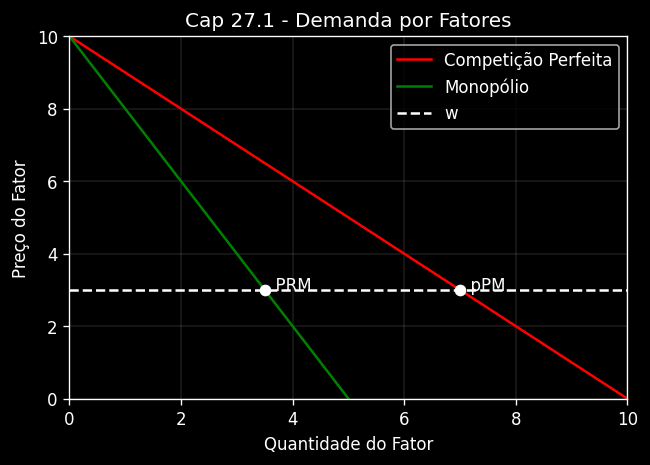
\includegraphics[scale=0.75]{cap27_1-demanda_fatores.png}
\end{figure}

\section{O Monopsônio}

O livro constrói um cenário onde temos um mercado competitivo de fatores, um único comprador e um mercado de produtos competitivo.
\\
\\
Para simplificar, vamos supor que a empresa usa apenas um único fator de produção. Sua função de produção será dada por $y = f(x)$.  A análise de comportamento do monopsônio é parecida com a do monopólio, só que ao invés de impactar o mercado pela oferta de bens, o poder de mercado é exercido pela compra. A quantidade de fator comprado, impactará no preço pago por ele.
\\
\\
Para expandir o modelo, vamos criar uma função de oferta inversa $w(x)$ onde o preço pago pelo insumo será determinado pela quantidade demandada pelo nosso único comprador (chamado de \textbf{monopsonista}). É razoável supor que $\frac{d w(x)}{d x} > 0$.
\\
\\
Como na imagem da seção acima, num mercado de fatores competitivo, a curva de oferta de fatores é plana. Ou seja, não importando a quantidade demanda, o custo será sempre o mesmo. Já no caso de um único comprador, a curva de oferta de fatores será inclinada positivamente. Como o professor resume perfeitamente: "Uma empresa num mercado de fatores competitivo é uma \textbf{tomadora de preços}. Um monopsionista é um \textbf{fixador de preços}".
\\
\\
A maximização de lucro do monoposionista será:

\begin{center}
\LARGE $\stackrel{máx}{\text{\small $x$}} \ \ \stackrel{pf(x) - w(x)x}{\ }$ \\
\end{center}

Ou seja, temos que encontrar a quantidade de insumo - $x$ - que permita maximizar a diferença entre a receita total - $p f(x)$ - e o custo total - $w(x)x$. A condição de primeira ordem desse problema será:

$$ pf'(x) - [ w(x) + w'(x)x ] = 0 $$
$$ pf'(x) = w(x) + w'(x)x $$
$$ \underbrace{pPM_x}_{\textrm{PRM}} = \ \underbrace{w(x) + w'(x)x}_{\textrm{Custo Marginal}} $$
\\
Como supomos no início do nosso caso, o mercado do produto é competitivo. Isso quer dizer que a receita marginal será igual a $pPM_x$ (que é a mesma coisa que $pf'(x)$). Mas obter o custo marginal não será tão simples quanto antes.
\\
\\
Quando a firma compra uma pequena quantidade ($x$) do fator de produção, ela deve pagar o preço desse fator vezes a quantidade ($wx$). Contudo, nesse caso, o preço será afetado exatamente na quantidade demanda ($w'(x)x$). O valor final pago é a soma dessas duas ações. Podemos desenvolver essa lógica exatamente como desenvolvemos a receita do monopolista na seção 25.1.

\newpage

$$ \Delta c = w \Delta x + x \Delta w $$
$$ \frac{\Delta c}{\Delta x} = w + x \frac{\Delta w}{\Delta x} $$
$$ = w \left[ 1 + \frac{x}{w} \frac{\Delta w}{\Delta x} \right] $$
$$ = w \left[1 + \frac{1}{\eta} \right] $$
\\
Onde $\eta$\footnote{O nome dessa letra grega é eta.} representa a elasticidade da oferta. Como a inclinação a curva de oferta é positiva, $\eta$ será maior que zero. Se a elasticidade da oferta for perfeita, $eta$ será infinito. O que implica, por sua vez, no caso da competição perfeita onde o custo marginal seria igual a $w$. Quaisquer outro valor da elasticidade, produzirá uma curva de oferta não plana.

\subsection{Monopsônio com Oferta Linear}

Para aplicar a teoria precisamos dar alguma forma funcional a nossa curva de oferta do fator de produção. No livro, o professor trabalha com uma oferta linear da seguinte forma:

$$ w(x) = a + bx $$
\\
O custo total da produção será dado por:

$$ C(x) = w(x)x = ax + bx^2 $$
\\
O custo marginal do fator é obtido pela derivada da função custo total em relação ao fator $x$.

$$ CMa_x(x) = a + 2bx $$
\\
Graficamente, a quantidade do insumo demandado será igual ao ponto onde o $PRM = pPM$ é igual ao custo marginal da aquisição do insumo.

\begin{figure}[H]
\centering
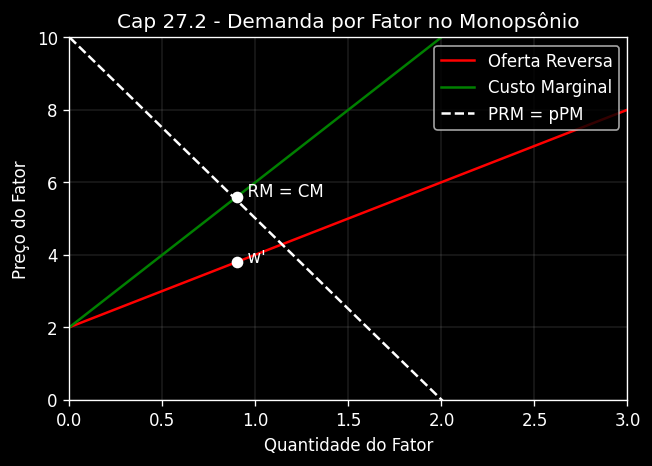
\includegraphics[scale=0.75]{cap27_2-demanda_fatores_monopsonio.png}
\end{figure}

Se o custo marginal for maior que o retorno da receita oriunda do emprego desse fator, o monopsionista não terá o incentivo à utilização do mesmo. Caso o contrário, valerá a pena usar um pouco mais do insumo. O ponto onde não há incentivo a mudança é justamente onde o custo marginal é igual à receita marginal.
\\
\\
Assim como no caso do monopolista, a quantidade demanda será o ponto menor do que se o mercado fosse competitivo. No cenário de competição, a quantidade demandada seria o ponto onde a oferta reversa se equivalesse ao retorno do emprego do insumo (medido pelo $PRM$). Só que nesse caso, a ineficiência acontece no mercado de fatores e não no de produção.
\\
\\
\textbf{Comentário:} Veja o exemplo sobre o salário mínimo que o professor colocou no livro. Você deve ser capaz de entendê-lo sem tanto sofrimento. A conclusão de que no mercado de trabalho controlado por um monopsionista, um salário mínimo pode aumentar o nível de emprego é bem interessante.

\section{Monopólios Upstream e Downstream na Cadeia de Produção}

Nós só observamos dois tipos de concorrência imperfeita. Mas os exemplos acima são apenas um dos múltiplos arranjos que podem acontecer na realidade. O professor não achou serventia em ter que modelar todas as cominações possíveis, e eu não vou fazer isso também. O importante é saber como modelar o comportamento do monopolista (ou do monopsionista) seja no mercado de fatores ou no mercado de produção.
\\
\\
Mesmo não querendo modelar todos os arranjos possíveis, ainda veremos uma nova situação: O caso onde um monopolista no mercado de fatores vende para um monopolista no mercado de produção.
\\
\\
O monopolista do mercado de fatores é chamado de \textbf{upstream} ou \textbf{para trás}. Ele vende o insumo $x$ ao preço $k$ e com custo marginal constante $c$. O monopolista do mercado de produto será denominado por \textbf{downstream} ou \textbf{para frente}. Esse segundo usará o insumo $x$ para obter a produção  $y$ via função de produção da forma $f(x) = y$ que será vendida no mercado cuja demanda inversa será $p(y)$. No nosso exemplo a forma funcional dessa demanda será $p(y) = a - by$.
\\
\\
O professor usa uma simplificação bem camarada da função de produção do downstream. Ele supõe que $f(x) = y = x$, ou seja, é como se ele revendesse o produto\footnote{O que torna esse exemplo surpreendentemente válido para diversas ocasiões da vida real.}. Outra simplificação é que o downstream também terá custo marginal igual ao preço pago pelo insumo ($k$) ao upstream.
\\
\\
Teremos que buscar um equilíbrio entre os dois monopolistas. Para isso, vamos começar modelando o caso para o downstream. Ele quer maximizar seu lucro que é dado pelo seguinte problema:

\begin{center}
\LARGE $\stackrel{máx}{\text{\small $y$}} \ \ \stackrel{L(y)\ =\ p(y)y - ky}{\ }$ \\
\end{center}
\begin{center}
\LARGE $\stackrel{máx}{\text{\small $y$}} \ \ \stackrel{L(y)\ =\ [a - by]y - ky}{\ }$ \\
\end{center}
\begin{center}
\LARGE $\stackrel{máx}{\text{\small $y$}} \ \ \stackrel{L(y)\ =\ ay - by^2 - ky}{\ }$ \\
\end{center}

A condição de primeira ordem da última forma é dada por:

$$ \frac{d L(y)}{d y} = a - 2by - k = 0 $$
$$ a - 2by = k $$
$$ y = \frac{a - k}{2b} $$

Como a função de produção usada iguala a quantidade de insumo à quantidade de produto. Vemos que ele demandará exatamente a mesma quantidade de fator de produção que a oferta no mercado do produto.

$$ x = \frac{a - k}{2b} $$

\textbf{Comentário:} O importante aqui é perceber que a função de produção do monopolista downstream é usada para derivar a demanda do fator produzido pelo upstream. Perceba que a quantidade demandada de fator depende do preço pago por ele e da demanda no mercado de produto. Tudo bem intuitivo e simples.
\\
\\
Agora temos que modelar o comportamento do upstream. Vamos supor que ele tenha acesso à função demanda de fatores do downstream e queira maximizar seu lucro. A demanda inversa de fatores nada mais é do que a última equação tendo k em função de x:

$$ k(x) = a - 2bx $$

A receita é dada por:

$$ k(x)x = ax - 2bx^2 $$

E a receita marginal por:

$$ RM_x = a - 4bx $$

Igualando a receita marginal ao custo marginal, teremos que:

$$ a - 4bx = c $$

ou seja, o total vendido no mercado pelo monopolista upstream será dado por:

$$ x = \frac{a - c}{4b} $$

Como a função de produção é um pra um, podemos definir que o total produzido no mercado de produto será:

$$ y = \frac{a - c}{4b} $$

Essa é a quantidade da produção que maximiza os lucros do monopolista upstream. Mas lembre-se que ele usa como função de demanda de fatores o resultado do problema de maximização do downstream. Então a solução acaba por gerar um lucro fruto do processo de maximização de ambos os monopolistas.
\\
\\
Se houvesse apenas um monopolista em ambos os mercados (imagine que as duas empresas se fundissem) e os custos de produção dos fatores se mantivessem os mesmos. O problema de maximização seria igualar a receita marginal ($a - 2by$) ao custo do fator ($c$). Isso geraria um volume de produção igual à

$$ y_{int} = \frac{a - c}{2b}$$
\\
O monopolista integrado produzirá o dobro que o arranjo com dois monopolistas separados. Mas qual o motivo dessa diferença?
\\
\\
Para entendermos o motivo dessa diferença precisamos lembrar que o monopolista sempre escolherá o ponto que maximiza o seu lucro pela igualdade entre o custo marginal e a receita marginal. A curva de demanda inversa do mercado serve para determinar o preço de equilíbrio que será usado no mercado dada a decisão da quantidade da produção do monopolista.
\\
\\
O caminho usado para encontrarmos o equilíbrio teve uma etapa para cada monopolista:
\begin{itemize}

\item Primeiro usamos a demanda do mercado de produtos para determinar qual a quantidade o monopolista ofertará (e como essa quantidade é função do preço do fator de produção).

\item Depois, usamos a relação entre a quantidade produzida e os insumos para determinar a demanda inversa do mercado de fatores. Essa demanda é usada pelo monopolista upstream para determinar o seu ponto de maximização.

\end{itemize}

Na prática, o monopolista upstream vai cobrar uma quantidade cujo preço de mercado é superior ao custo marginal. Esse preço será o custo que o monopolista downstream usará para maximizar seu lucro. Contudo, quando as empresas se fundem, o novo custo marginal do monopolista do mercado de produto será exatamente o custo de produção $c$. Nós retiramos de cena o Markup do monopolista upstream.

%%%%%%%%%%%%%%%%%%%%%%%% CHAPTER %%%%%%%%%%%%%%%%%%%%%%%%
\chapter{O Oligopólio}

\begin{chapquote}{The Godfather}
	``I want you to talk to this movie bigshot and settle this business for Johnny. Now, if there's nothing else, I'd like to go to my daughter's wedding.''
\end{chapquote}


O trabalho de entender os mercados é longo e trabalhoso. Até agora, nós elaboramos as estruturas mais simples e que se encontram nos dois extremos do poder de mercado. De um lado, aprendemos a estrutura onde não existe poder de mercado e as empresas são pequenas concorrentes. Após isso, vimos o que acontece quando temos apenas uma empresa (ou empresas que trabalham como se fossem uma só) e o poder de mercado está todo nas mãos dela.
\\
\\
Agora vamos entrar num cenário um pouco mais realista. Pensemos em uma situação onde temos poucos concorrentes. De um lado, não temos tantos a ponto de ninguém poder manipular seus preços. Do outro, ninguém é grande o suficiente para ignorar o comportamento dos seus concorrentes. Esse arranjo é denominado de \textbf{Oligipólio}.
\\
\\
Nós já tangenciamos esse assunto quando vimos o modelo de concorrência monopolística no capítulo 25. Esse arranjo também é um tipo de oligopólio. Nessa configuração, as variáveis mais importantes são o custo de entrada (pela regra do custo médio) e nas estratégias de diferenciações entre os produtos (seja a de convergência ou a de diferenciação).
\\
\\
Aqui vamos estudar arranjos com um número ainda menor de concorrentes. Como dito anteriormente, a medida que aprimoramos o nosso modelo, as características únicas de cada mercado se tornam cada vez mais relevantes. Aqui só vamos conseguir ver regras gerais de resultados possíveis, bem como, algumas variáveis importantes para monitorarmos.
\\
\\
Vamos partir da estrutura de competição de apenas duas empresas: o \textbf{Duopólio}\footnote{Alguns exemplos em que podemos aproximar esse modelo: PS4 x Xbox, Iphone x Samsung, Coca-Cola x Pepsi, Apple x Microsoft.}. Outra limitação que imporemos é a de que os produtos são idênticos. Essas limitações nos livram de notações complexas com várias competidores e a utilização do poder de mercado oriundo da diferenciação. Nosso foco são as \textbf{interações estratégicas}.\footnote{Se você quiser ver modelos mais próximos da realidade, vai ter que encarar um mestrado e um doutorado.}

\section{A Escolha de Uma Estratégia}

Em um arranjo de dois competidores, temos que desenvolver um modelo que consiga equilibrar 4 variáveis:

\begin{itemize}
\item Preço da Empresa 1
\item Preço da Empresa 2
\item Quantidade da Empresa 1
\item Quantidade da Empresa 2
\end{itemize}

Na hora de tomar uma decisão sobre o preço e a quantidade, uma empresa pode, ou não, ter acesso as escolhas feitas pelo seu concorrente. Chamaremos de \textbf{líder} toda empresa que decidir seu \textbf{preço} ou \textbf{quantidade} antes da outra. A empresa que decidirá após a informação da decisão da empresa líder será chamada de \textbf{seguidora}. As interações desse tipo são chamadas de \textbf{jogos sequenciais}.\footnote{Começamos a chegar mais perto da teoria dos jogos.}
\\
\\
Quando as duas empresas decidem sem ter acesso a informação do adversário, elas precisam supor o que ele fará. Esse arranjo é denominado \textbf{jogo simultâneo}.
\\
\\
Com esses dois conceitos, podemos ter 4 tipos de interações estratégicas:

\begin{itemize}
\item Liderança de Preço
\item Liderança de Quantidade
\item Preço Simultâneo
\item Quantidade Simultânea
\end{itemize}

Analisaremos cada tipo de interação estratégica que surge com cada tipo de esquema. Mas não pararemos ai. Uma opção possível de estratégia é a de negociação entre as empresas para formação de um \textbf{conluio}. Esse tipo de esquema é chamado de \textbf{jogo cooperativo}.
\\
\\
\textbf{Comentário:} Leia o exemplo da estratégia de "cobrimos o preço da concorrência"\ e a partir de agora, você nunca mais lerá essas ofertas com os mesmos olhos.

\section{Liderança de Quantidade}

O modelo desenvolvido nessa seção é creditado ao economista alemão Heinrich von Stackelberg. Seu livro \textit{Marktform und Gleichgewicht} foi publicado em 1934.\footnote{Eu recomendo dar uma olhada na bibliografia dos gigantes que desenvolveram as teorias ao longo desse livro.}.
\\
\\
Vamos supor que temos uma empresa líder na quantidade. Como é de se esperar, ela fixará sua produção em $y_1$ unidades. A empresa seguidora, de posse da informação de $y_1$ e da demanda inversa do mercado, escolherá seu nível de produção em $y_2$. A demanda inversa do mercado será em função do total de produtos $p(Y) = p(y_1 + y_2)$.
\\
\\
Como a empresa líder decidirá sua quantidade de modo a maximizar seus lucros? Certamente ela terá que supor como a empresa seguidora agirá. Não seria nada estranho que ela tivesse a hipótese que a empresa seguidora queira maximizar seus lucros também . Desse modo, a empresa líder terá que endogenizar o problema da maximização do lucro da empresa seguidora.

\subsection{O Problema da Empresa Seguidora}

O problema da maximização da empresa seguidora é:

\begin{center}
\LARGE $\stackrel{máx}{\text{\small $y_2$}} \ \ \stackrel{p(y_1 + y_2)y_2 - c_2(y_2)}{\ }$ \\
\end{center}

Já conhecemos esse tipo de problema muito bem. Queremos encontrar o ponto onde a receita marginal será igual ao custo marginal.

$$ RM_2 + CMa_2 = p(y_1 + y_2) + \frac{dp(y_1+y_2)}{dy_2}y_2 + \frac{dc_2(y_2)}{y_2} = 0  $$

ou, na notação de derivadas de Lagrange

$$ RM_2 + CMa_2 = p(y_1 + y_2) + p'(y_1 + y_2)y_2 + c'(y_2) = 0  $$

A novidade aqui é que temos que levar em consideração a quantidade $y_1$ para encontrar nosso $y_2$. Isso quer dizer que 

$$y_2 = f_2(y_1)$$

Nós conseguimos obter essa função isolando nosso termo $y_2$ no problema de maximização acima. Essa função tem o nome de \textbf{função de reação} e nos diz qual quantidade será produzida pela empresa seguidora ao ser conhecida a quantidade da empresa líder.
\\
\\
Para prosseguirmos vamos ter que definir uma forma funcional à nossa função de demanda inversa. Faremos para o caso linear onde $p(y_1 + y_2) = a - b(y_1 + y_2)$. Também adotaremos o custo igual a zero para facilitar a matemática da coisa.

$$\textrm{Função Lucro 2: } \pi_2(y_1,y_2) = p(y_1 + y_2)y_2$$
$$ = [a - b(y_1 + y_2)]y_2 = ay_2 - by_1 y_2 - by_2^2 $$

Com a função de lucro e a de reação, conseguimos ver a relação entre essas duas funções. Na imagem abaixo podemos ver que a curva de reação sempre atravessa as curvas de isolucro no ponto onde temos o maior valor de $y_2$.

\begin{figure}[H]
\centering
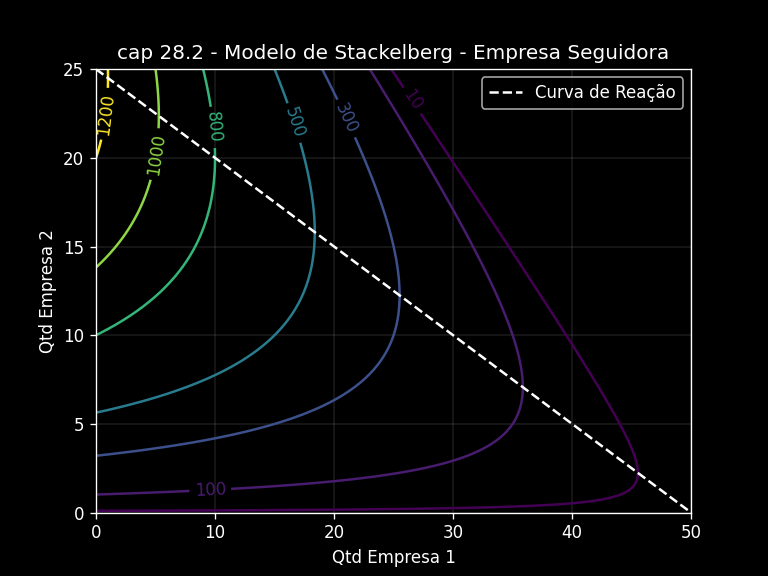
\includegraphics[scale=0.75]{cap28_2-modelo_stackelberg_parcial.png}
\end{figure}

\subsection{O Problema da Empresa Líder}

Já aprendemos a parte do modelo que trata da quantidade de equilíbrio dada a escolha anterior da empresa líder. Agora vamos desenvolver como essa empresa define a sua quantidade de modo a maximizar o seu lucro.
\\
\\
Uma das características desse modelo é que a empresa líder sabe como a outra empresa vai se comportar dada a escolha dela, ou seja, ela conhece $f_2(y_1)$. Diante disso, o problema da maximização dela está sujeita a essa restrição.

\begin{center}
\LARGE $\stackrel{máx}{\text{\small $y_1$}} \ \ \stackrel{p(y_1 + y_2)y_1 - c_1(y_1)}{\ }$ \\
\small de modo que \normalsize $y_2 = f_2(y_1)$
\end{center}

Ou melhor, podemos colocar tudo em função de $y_1$ e obtermos

\begin{center}
\LARGE $\stackrel{máx}{\text{\small $y_1$}} \ \ \stackrel{p[y_1 + f_2(y_1)]y_1 - c_1(y_1)}{\ }$ \\
\end{center}

A produção total será definida pela líder sendo que será parte devida a produção direta e a outra parte pela resposta da seguidora ao nível definido da produção, ou seja, $y_1 + f_2(y_1)$. Pela equação da demanda inversa linear, temos que a função de reação da empresa seguidora é

$$ f_2(y_1) = y_2 = \frac{a - by_1}{2b}$$

A função lucro é dada pela receita menos os custos (que no nosso exemplo é zero)

$$ \textrm{Função Lucro 1: } \pi(y_1,y_2) = [a - b(y_1 + y_2)]y_1 = ay_1 -by_1^2 - by_1y_2 $$

Colocando a função de reação dentro da função de lucro teremos

$$ = ay_1 -by_1^2 - by_1f(y_1)$$
$$ = ay_1 -by_1^2 - by_1\frac{a - by_1}{2b}$$
$$ = ay_1 -by_1^2 - \frac{\cancel{b}y_1a}{2\cancel{b}} + \frac{\cancel{b}*b(y_1)^2}{2\cancel{b}}$$
$$= ay_1 -by_1^2 - \frac{ay_1}{2} + \frac{by_1^2}{2}$$
$$ \pi(y_1,y_2) = \frac{a}{2}y_1 - \frac{b}{2}y_1^2$$

Para encontrarmos a quantidade ótima basta derivar a função lucro em função de $y_1$ e igualar a zero. O que nos dará 

$$ y_1^* = \frac{a}{2b} $$

Desse modo, podemos encontrar facilmente a produção de equilíbrio da empresa seguidora.

$$ y_2^* = \frac{a - by_1}{2b} $$
$$ y_2^* = \frac{a - b(a/2b)}{2b} $$
$$ y_2^* = \frac{a - ab/2b}{2b} $$
$$ y_2^* = \frac{2ab/2b - ab/2b}{2b} $$
$$ y_2^* = \left( \frac{2ab}{2b} - \frac{ab}{2b} \right) \frac{1}{2b} $$
$$ y_2^* = \left( \frac{\cancel{2}a\cancel{b}}{\cancel{2b}} - \frac{a\cancel{b}}{2\cancel{b}} \right) \frac{1}{2b} $$
$$ y_2^* = \left( a - \frac{a}{2} \right) \frac{1}{2b}$$
$$ y_2^* = \frac{a}{4b} $$

Por fim, podemos ter a quantidade total do mercado pela soma de $y_1^* + y_2^* = \frac{3a}{4b}$. Agora que temos a função de lucro da empresa 1, podemos acrescentar as curvas de isolucro para vermos a solução gráfica da álgebra que acabamos de desenvolver.

\begin{figure}[H]
\centering
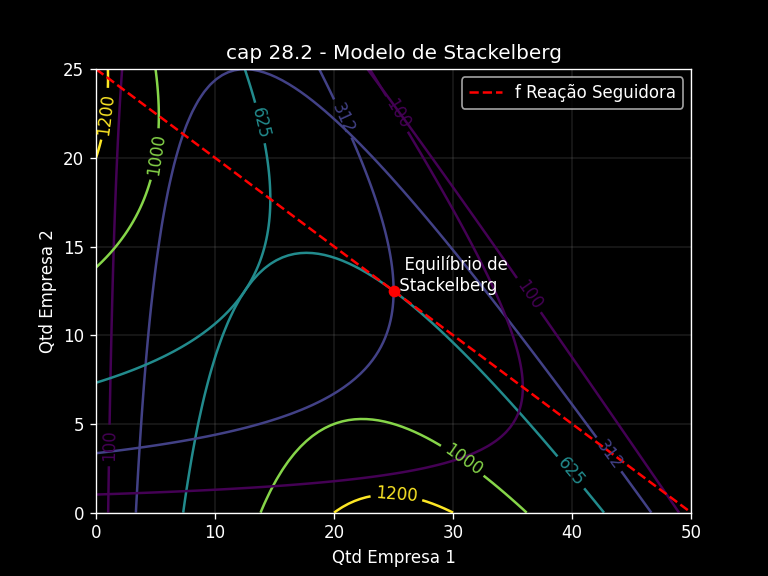
\includegraphics[scale=0.75]{cap28_2-modelo_stackelberg_completo.png}
\end{figure}

Se você colocar as quantidades de equilíbrio nas equações de lucro, chegará nos valores de lucro para cada empresa desse modelo. O ponto de Equilíbrio de Stackelberg acontecerá onde a curva de reação tangencia a maior curva de isolucro da empresa líder. No exemplo da imagem eu usei para a função da demanda inversa linear um $a = 100$ e um $b = 2$.

\section{Liderança do Preço}

Outra forma de um jogo sequencial acontecer entre duas empresas é pela definição do preço pela empresa líder. Similarmente ao que vimos na seção anterior, a empresa líder precisa levar em consideração o que a empresa seguidora fará.

\subsection{O Problema da Seguidora}
No mercado competitivo, o preço é dado e as empresas maximizam seus lucros pela igualdade entre a a receita marginal (que é justamente o preço) e o custo marginal. Por sorte, o problema da empresa seguidora é bem parecido com esse. Ela recebe o preço definido pela líder e maximiza seu lucro.

\begin{center}
\LARGE $\stackrel{máx}{\text{\small $y_2$}} \ \ \stackrel{py_2 - c_2(y_2)}{\ }$ \\
\end{center}

A oferta da empresa seguidora será a quantidade que iguala o preço definido pela líder ao custo marginal.

\subsection{O Problema da Líder}

A empresa líder, sabendo a função de oferta da empresa seguidora, vai trabalhar com a diferença entre a Demanda do mercado e a demanda da empresa seguidora, ou seja, $R(p) = D(p) - S(p)$. O nome dessa curva de demanda reduzida é \textbf{curva de demanda residual}.
\\
\\
Supondo um custo de produção constante $c$. A função de lucro da empresa líder é dada por

$$ \textrm{Função Lucro 1: } \pi_1(p) = R(p)p - R(p)c = (p - c)R(p)  $$

A maximização dessa empresa acontece onde a receita marginal (que nesse caso é oriunda da demanda residual) é igual ao custo marginal. 
\\
\\
A partir de agora temos que definir uma forma funcional para a nossa curva de demanda, como sempre, vamos optar pelo caso mais simples, $D(p) = a - bp$. Também vamos definir as funções custo para a seguidora $c_2(y_2) = y_2^2/2$ e para a líder $c_1(y_1) = cy_1$.
\\
\\
Isso nos diz que a condição de maximização da empresa seguidora será a derivada da função lucro igual a zero.

$$ \frac{d L(y_2)}{y_2} = p - \frac{2y_2}{2} = 0 $$
$$ = p - y_2 = 0 $$
$$ = p = y_2 $$

Ou seja, nossa função de oferta da seguidora será $S(p) = p$. De posse dessa informação, podemos descobrir a equação da demanda residual da empresa líder pela subtração da curva de demanda pela oferta da seguidora.

$$ R(p) = D(p) - S(p) = a - bp - p = a - (b + 1)p $$

Agora é só maximizar o lucro pela igualdade entre a receita marginal e o custo marginal e verificar na curva de demanda inversa o volume de produção e o preço. A demanda inversa é obtida isolando $p$ da demanda residual.

$$ p(y_1) = \frac{a}{b+1}-\frac{1}{b+1}y_1 $$

A receita da empresa líder é obtida pela multiplicação de $p(y_1)$ por $y_1$. A receita marginal é a derivada dessa função em relação a $y_1$.

$$ Receita_1: \left[ \frac{a}{b+1} - \frac{1}{b+1}y_1 \right] y_1 $$
$$ = \frac{a}{b+1}y_1 - \frac{1}{b+1}y_1^2 $$

A receita marginal será

$$ RMa_2 = \frac{a}{b+1} - \frac{2}{b+1}y_1 $$

O nosso custo foi definido como $c_1(y_1) = cy_1$, logo, o custo marginal é igual a $c$\footnote{A essa altura do campeonato você não tem mais dúvida nessas derivadas triviais né?!}.
\\
\\
Portanto, nosso problema de maximização será dado pela equação

$$ \frac{a}{b+1} - \frac{2}{b+1}y_1 = c $$
$$ - \frac{2}{b+1}y_1 = c - \frac{a}{b+1} $$
$$ \frac{2}{b+1}y_1 = \frac{a}{b+1} - c $$
$$ \frac{2}{b+1}y_1 = \frac{a}{b+1} - \frac{c(b+1)}{b+1} $$
$$ \frac{2}{\cancel{b+1}}y_1 = \frac{c(b+1)}{\cancel{b+1}} $$
$$ 2y_1 = c(b+1) $$
$$ y_1^* = \frac{c(b+1)}{2} $$

Na imagem abaixo, nós podemos ver as variáveis interagindo. A oferta total será a soma das quantidades de ambas empresas.

\begin{figure}[H]
\centering
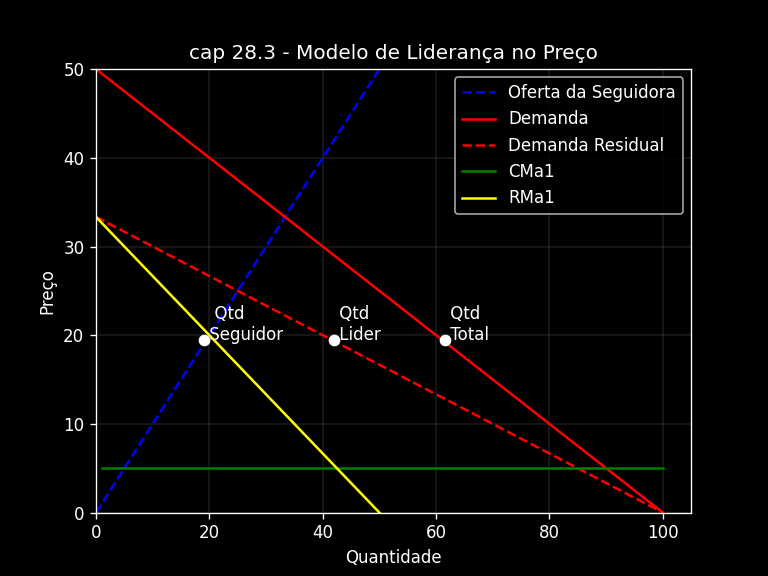
\includegraphics[scale=0.75]{cap28_3-lideranca_preco.png}
\end{figure}

\section{Comparação entre as Lideranças de Preço e Quantidade}

Esse seção do livro é bem explicativa. Vá ler o material original.

\section{Estabelecimento Simultâneo da Quantidade}

Não raramente, as empresas não ficam se comunicando entre si para informar seus concorrentes a respeito de suas decisões . Nesses cenários, as empresas precisam supor o que suas concorrentes farão. Esse modelo é chamado de \textbf{Modelo de Cournot} e é um modelo de jogo simultâneo onde as empresas definem suas quantidades produzidas e vendidas no mercado.
\\
\\
Como de costume, suporemos que as empresas queiram maximizar seus lucros. Pensemos no caso da empresa 1. A quantidade total do mercado será dada por $Y = y_1 + y_2^e$, onde $y_2^e$ é a quantidade prevista da empresa 2. O preço de equilíbrio do mercado será dado pela equação de demanda inversa $p(Y) = p(y_1 + y_2^e)$.
\\
\\
O problema de maximização do lucro será

\begin{center}
\LARGE $\stackrel{máx}{\text{\small $y_1$}} \ \ \stackrel{p(y_1 + y_2^e)y_1 - c(y_1)}{\ }$ \\
\end{center}

Não é difícil ver que quaisquer expectativa da produção da sua concorrente mudará o ponto de produção que maximizaria o lucro. Desse modo, podemos ver que existe uma relação entre essa expectativa e a produção, de modo mais formal, $y_1 = f(y_2^e)$.
\\
\\
Mas, espera um pouco, a gente já viu algo bem parecido um pouco mais acima. Essa é a \textbf{curva de reação} da empresa, a diferença é que aqui a empresa 1 não é mais a líder e essa reação se refere a \textit{expectativa} da produção. Mas o tratamento matemático é o mesmo.\footnote{Para a nossa sorte!}
\\
\\
Similarmente, a empresa 2 se depara com a mesma situação.

$$y_2 = f(y_1^e)$$

Como ambas maximizações são funções de expectativas, é muito mais provável que as empresas não acertem exatamente o volume de produção da sua concorrente. O equilíbrio de Cournot é dado pelo sistemas de equações

$$ y_1^* = f_1(y_2^*) $$
$$ y_2^* = f_2(y_1^*) $$

Nessa solução, nenhuma das empresas terá incentivos em mudar seu nível de produção.

\section{Exemplo do Equilíbrio de Cournot}

Se reutilizarmos o exemplo na liderança da quantidade (com custo zero e demanda linear) obteremos as mesmas funções de reação que a empresa 2 tinha naquele modelo.

$$ y_1 = \frac{a - by_2^e}{2b} $$

e

$$ y_2 = \frac{a - by_1^e}{2b} $$

O ponto de equilíbrio acontece onde $y_1 = y_2$, ou seja, onde as curvas de reação são iguais. Nesse ponto, $y_1^e = y_1$ e $y_2^e = y_2$. Só precisamos substituir dentro desse sistema de equações do seguinte modo

$$ y_1 = \frac{a - by_2^e}{2b} $$
$$ y_1 = \frac{a - by_2}{2b} $$
$$ y_1 = \frac{a - b(\frac{a - by_1}{2b})}{2b} $$
$$ y_1 = \frac{a - (\frac{ab - b^2y_1)}{2b})}{2b} $$
$$ y_1 = \frac{\frac{2ba}{2b} - (\frac{ab - b^2y_1)}{2b})}{2b} $$
$$ y_1 = \frac{2ba - ab + b^2y_1}{2b}\frac{1}{2b} $$
$$ y_1 = \frac{2ba - ab + b^2y_1}{4b}\frac{1}{b} $$
$$ y_1 = \frac{2\cancel{b}a - a\cancel{b} + b^{\cancel{2}}y_1}{4\cancel{b}}\frac{1}{b} $$
$$ y_1 = \frac{2a - a + by_1}{4b} $$
$$ 4by_1 - by_1 = a $$
$$ 3by_1 = a $$
$$ y_1^* = \frac{a}{3b} = y_2^* $$

Com essas funções e as equações de lucro podemos ver graficamente o equilíbrio de Cournot onde as curvas de reação se equivalem.

\begin{figure}[H]
\centering
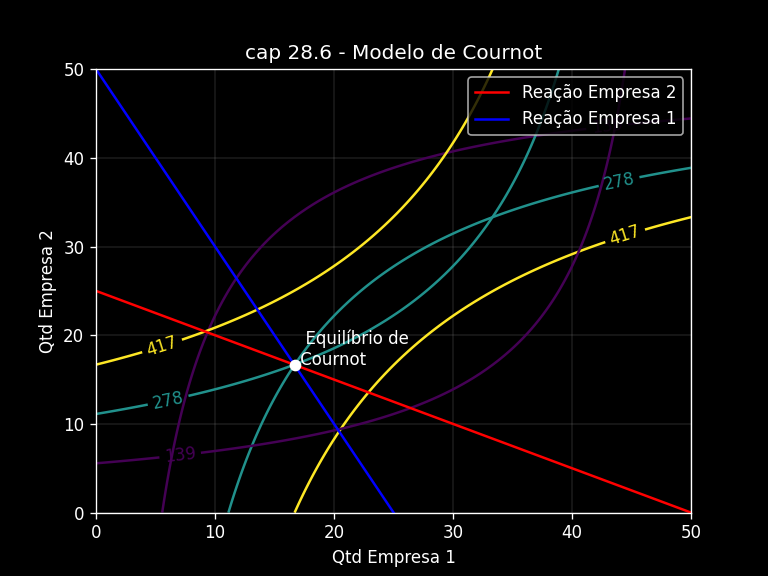
\includegraphics[scale=0.75]{cap28_6-modelo_cournot.png}
\end{figure}

\section{Ajustamento para o Equilíbrio}

Seria muita boa vontade supor que, na vida real, as empresas conseguissem acertar na mosca o nível de produção dos seus concorrentes. Mas o nosso modelo é forte o suficiente para um processo de ajustamento em caso de (prováveis) palpites equivocados no nível de produção.
\\
\\
Imaginemos que as empresas suponham que a produção do seu concorrente será uma quantidade qualquer diferente do equilíbrio. Para facilitar, vamos supor que a cesta inicial produzida esteja em cima da curva de reação da empresa 2. A cesta inicial, que chamamos no gráfico de $Cesta(t)$ será igual à lista $(y_1^t,y_2^t)$.
\\
\\
Essa cesta está na curva de reação da empresa 2, logo, essa empresa não terá incentivo a fazer nenhuma mudança. Mas para a empresa 1, a situação é outra, ela quer reduzir sua produção para aumentar seus lucros.
\\
\\
Isso faz com que a cesta do mercado se desloque para a curva de reação da empresa 1. Mas agora, quem está insatisfeito é a empresa 2. Ela fara um reajuste, só que agora, usará a nova produção da empresa 1 para definir sua oferta.
\\
\\
Esse processo fica se realimentando até um ponto onde elas estão satisfeitas. Nós já vimos agora a pouco que esse ponto é justamente o equilíbrio do modelo de Cournout.
\\
\\
A imagem abaixo mostra esse caminho. Mas eu também transformei ela em um gif animado\footnote{Com alguma dose de bom humor.} para ilustrar o caminho até o equilíbrio.

\begin{figure}[H]
\centering
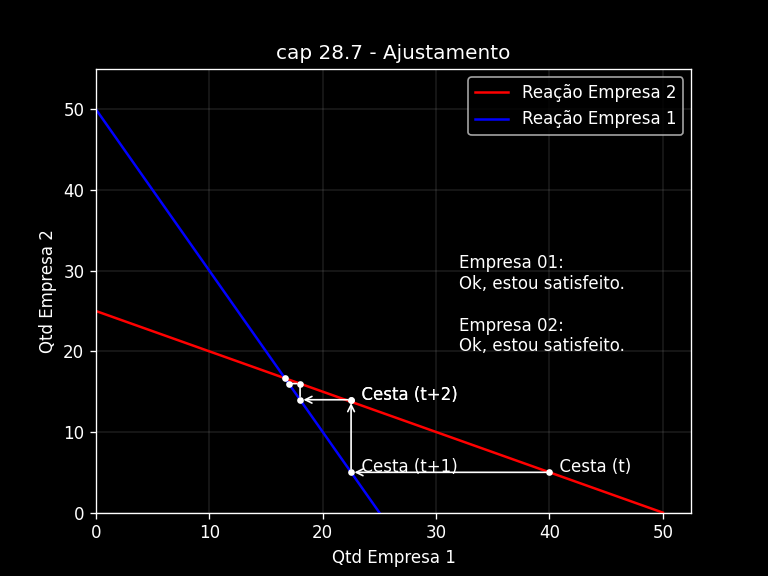
\includegraphics[scale=0.75]{cap28_7-ajustamento.png}
\end{figure}

Essa propriedade de convergência ao ponto de equilíbrio é o que caracteriza esse modelo como um modelo de \textbf{equilíbrio estátvel}. Embora o processo descrito aqui seja bem resumido e simplificado devido o escopo do nosso curso.

\section{Várias Empresas no Equilíbrio de Cournot}

Além de fornecer um modelo para um duopólio, podemos ajustar o modelo de Cournot para $n$ empresas competidoras. A oferta total da indústria será dada por $Y = y_1 + y_2 + \dots + y_{n-1} + y_n$. Desse modo o problema da maximização da empresa será dado pela igualdade entre a receita marginal e o seu custo marginal do seguinte modo

$$ p(Y) + \frac{\delta p}{\delta Y} y_i = CMa(y_i) $$
$$ p(Y) + \frac{\delta p}{\delta Y} \frac{Y}{Y} \frac{p(Y)}{p(Y)} y_i = CMa(y_i) $$
$$ p(Y) \left[1 + \frac{\delta p}{\delta Y} \frac{Y}{p(Y)} \frac{y_i}{Y} \right] = CMa(y_i) $$

Definindo $s_i = \frac{y_i}{Y}$ como a participação da empresa no total do mercado.

$$ p(Y) \left[1 + \frac{\delta p}{\delta Y} \frac{Y}{p(Y)} s_i \right] = CMa(y_i) $$

O termo $p(Y)$ é a curva de demanda. Então, se lembrarmos da fórmula da elasticidade, podemos ver que o termo $\frac{\delta p}{\delta Y} \frac{Y}{p(y)}$ é justamente o inverso da elasticidade $\frac{1}{\epsilon(Y)}$

$$ p(Y) \left[1 + \frac{s_i}{\epsilon(Y)} \right] = CMa(y_i) $$

Como a elasticidade de demanda é negativa

$$ p(Y) \left[1 - \frac{s_i}{|\epsilon(Y)|} \right] = CMa(y_i) $$

O professor faz uma transformação que, para alguns, pode parecer estranha. Mas a lógica é essa (se tiver difícil de ver, dá um zoom):

$$ \frac{1}{\frac{\epsilon(Y)}{s_i}} = \frac{\frac{1}{1}}{\frac{\epsilon(Y)}{s_i}} = \frac{1}{1} \frac{s_i}{\epsilon(Y)} = \frac{s_i}{\epsilon(Y)} $$

Com essa transformação, chegamos em

$$ p(Y) \left[1 - 1/\frac{|\epsilon(Y)|}{s_i} \right] = CMa(y_i) $$

Essa solução é bem parecida com a maximização do monopolista. A principal diferença é esse termo $s_i$ dividindo a elasticidade. Como $s_i = y_i/Y$ ele será $0 \leq s_i \leq 1$. No caso monopolista, sabemos que $s_i = 1$. No outro extremo, se $lim (s_i) \rightarrow 0$, a empresa terá elasticidade infinita como as empresas da competição perfeita.  
\\
\\
Para as empresas não monopolísticas e com algum poder de mercado, podemos entender esse termo como a elasticidade da demanda da empresa. Quanto maior $s_i$ menor será a elasticidade da demanda da empresa.
\\
\\
Isso nos mostra que, em um mercado competitivo, temos um equilíbrio de Cournot. As empresas estarão maximizando seus lucros sem incentivo em mudar seu nível de produção.

\section{Fixação Simultânea de Preços}

Da mesma maneira que conseguimos desenvolver um modelo para quantidade e preço em jogos sequenciais, podemos fazê-lo para os jogos simultâneos. Já aprendemos nessa última seção como as empresas definem as quantidades produzidas de modo a maximizar seus lucros sem que haja uma empresa líder no processo.
\\
\\
Acontece que, em algum momento do século XIX, um matemático francês de nome Joseph Bertrand, ao ler o livro do Cournot, desenvolveu um modelo simultâneo de equilíbrio de preços. Esse modelo ficou conhecido como \textbf{concorrência de Bertrand}.
\\
\\
Assim como fizemos com Cournot, estamos na busca do par de preços que permitam ambas as empresas maximizar seus lucros. Para isso, temos que seguir algumas regras que já fazem parte dos modelos usados até o momento ao longo de todo o livro:

\begin{itemize}
\item O preço não poderá ser maior que o custo marginal. Porque as empresas aumentariam seus lucros simplesmente produzindo menos.
\item Se o preço for maior que o custo marginal, todas as empresas terão um incentivo de reduzir seu preço para "roubar"\ os clientes das concorrentes e ainda auferir lucros positivos.
\end{itemize}

O segundo ponto funciona de maneira recursiva. Se uma empresa reduz seu preço em $10\%$ abaixo dos preços das suas concorrentes, ela ganhará parte do mercado. As concorrentes terão o incentivo em reduzir mais ainda seus preços até o ponto onde não poderão mais reduzir (determinado pelo custo marginal).

\section{Conluio}	

Até agora, todas as soluções envolveram processos de competição entre as empresas. Contudo, não seria nem um pouco alheio à realidade supor que algumas empresas queiram operar de modo coordenado. Esse arranjo é chamado de \textbf{Cartel} e é crime em vários países.
\\
\\
Você já sabe, desde o capítulo 25, que um cartel não passa de um grupo de empresas se comportando como um monopolista. Diante disso, seu problema de maximização será muito parecido com o modelo do capítulo que tratamos sobre o monopólio.
\\
\\
O problema da maximização para um cartel de duas empresas será dado por

\begin{center}
\LARGE $\stackrel{máx}{\text{\small $y_1,y_2$}} \ \ \stackrel{p(y_1+y_2)[y_1 + y_2] - c_1(y_1) - c_2(y_2)}{\ }$ \\
\end{center}

Cujas condições de primeira ordem serão

$$p(y_1^* + y_2^*) + \frac{\delta p}{\delta Y}[y_1^* + y_2^*] = CMa_1(y_1^*)$$
$$p(y_1^* + y_2^*) + \frac{\delta p}{\delta Y}[y_1^* + y_2^*] = CMa_2(y_2^*)$$

Podemos ver que, quando uma empresa decide expandir sua produção, receberá uma quantia oriunda da venda dos seus produtos, contudo, essa oferta adicional reduzirá o preço de equilíbrio do mercado (o que reduz o lucro recebido). A novidade aqui é que essa redução do preço impactará também na outra empresa do cartel.
\\
\\
O que as duas equações anteriores nos dizem é que as quantidades produzidas (e ofertadas no mercado) serão as que igualem seus custos marginais $CMa_1(y_1^*) = CMa_2(y_2^*)$. 
\\
\\
Agora temos um fator interessante para pensarmos. Se uma empresa possuir uma estrutura de custos que permita produzir mais com o mesmo custo marginal que sua empresa companheira, ela obterá uma maior parte dos lucros do mercado. Uma vez que sua produção será maior.

\subsection{O problema da `Desonestidade'}

Será que as empresas que operam em um cartel possuem algum incentivo em "trapacear"\ a sua empresa parceita?\footnote{Nessas situações cabe o didato popular: "Ladrão que rouba ladrão tem ..."}
\\
\\
Vejamos o que acontece com a empresa 1 do nosso cartel, caso ela aumente a sua produção em $\delta y_1$ unidades. Podemos mensurar esse impacto pela derivada parcial da função lucro do cartal em relação a $y_1$

$$ \frac{\partial \pi_1}{\partial y_1} = p(y_1^* + y_2^*) + \frac{\delta p}{\delta Y}y_1^* - CMa_1(y_1^*) $$ 

A condição de maximização do cartel nos diz que

$$ p(y_1^* + y_2^*) + \frac{\delta p}{\delta Y}y_1^* + \frac{\delta p}{\delta Y}y_2^* - CMa_1(y_1^*) = 0 $$ 

Apenas isolando o termo referente à produção da empresa, temos então

$$ p(y_1^* + y_2^*) + \frac{\delta p}{\delta Y}y_1^* - CMa_1(y_1^*) = - \frac{\delta p}{\delta Y}y_2^* $$ 

Como $\delta p / \delta Y$ é negativo, então o termo da esquerda da última equação é positivo. Ou seja, a empresa 1 consegue aumentar seus lucros positivamente ao aumentar sua produção para além do ponto de equilíbrio do cartel.
\\
\\
Aqui mora o problema de longo prazo dos carteis. Na solução de maximização do lucro conjunto, existe um incentivo para cada empresa aumentar sua produção, visto que, se a outra empresa mantiver fixa a sua produção, sempre será lucrativo um aumento unilateral da quantidade produzida.
\\
\\
Agora, se houver desconfiança entre as empresas, fica mais difícil ainda manter a coalizão. Se as empresas esperam que a outra irá aumentar sua produção, elas terão um incentivo adicional em agir antes da outra e aproveitar os lucros positivos oriundos do aumento da produção.
\\
\\
Para exemplificar, vamos pegar uma demanda linear do tipo $p(Y) = a - b(y_1 + y_2)$ e supormos um custo marginal igual a $0$. A equação do lucro será dada por 

$$\pi(y_1,y_2) = p(Y)(y_1 + y_2) = [a - b(y_1 + y_2)](y_1 + y_2) = a(y_1 + y_2) - b(y_1 + y_2)^2$$

A condição de primeira ordem desse problema é dada pela derivada dessa função em relação a $(y_1 + y_2)$. O que nos dá

$$a - 2b(y_1 + y_2) = 0$$
$$y_1^* + y_2^* = \frac{a}{2b}$$

O gráfico abaixo ilustra exatamente esse situação para $a = 100, b = 2$ e os custos de produção fixos em $10$. Veja como temos 3 pontos onde as curvas de isolucro se tocam. Esses pontos ocorrem na reta de maximização do lucro dada pela equação acima.

\begin{figure}[H]
\centering
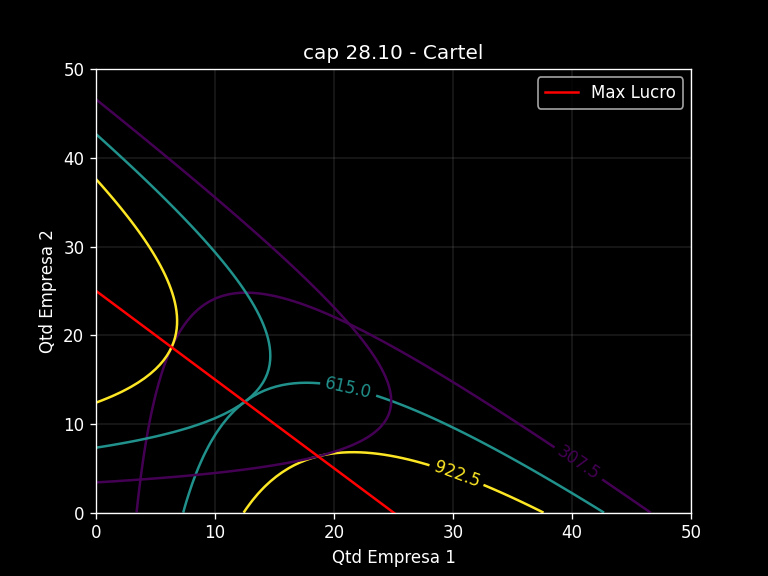
\includegraphics[scale=0.75]{cap28_10-cartel.png}
\end{figure}

Todas as soluções de maximização do lucro acontecem nas tangências das curvas de isolucro que ocorrem na reta de maximização. Quando uma empresa aumenta a produção unilateralmente, ela acaba deslocando o equilíbrio para um outro ponto dessa curva. Veja como a soma dos lucros nesses 3 pontos são iguais.

\section{Estratégias Punitivas}

\section{Comparação das Soluções}

%%%%%%%%%%%%%%%%%%%%%%%% CHAPTER %%%%%%%%%%%%%%%%%%%%%%%%
\chapter{A Teoria dos Jogos}

%%%%%%%%%%%%%%%%%%%%%%%% CHAPTER %%%%%%%%%%%%%%%%%%%%%%%%
\chapter{Aplicações da Teoria dos Jogos}

%%%%%%%%%%%%%%%%%%%%%%%% PART %%%%%%%%%%%%%%%%%%%%%%%%
\part{Tópicos Avançados}

%%%%%%%%%%%%%%%%%%%%%%%% CHAPTER %%%%%%%%%%%%%%%%%%%%%%%%
\chapter{Economia Comportamental}

%%%%%%%%%%%%%%%%%%%%%%%% CHAPTER %%%%%%%%%%%%%%%%%%%%%%%%
\chapter{Trocas}

%%%%%%%%%%%%%%%%%%%%%%%% CHAPTER %%%%%%%%%%%%%%%%%%%%%%%%
\chapter{Produção}

%%%%%%%%%%%%%%%%%%%%%%%% CHAPTER %%%%%%%%%%%%%%%%%%%%%%%%
\chapter{O Bem-Estar}

%%%%%%%%%%%%%%%%%%%%%%%% CHAPTER %%%%%%%%%%%%%%%%%%%%%%%%
\chapter{Externalidades}

%%%%%%%%%%%%%%%%%%%%%%%% CHAPTER %%%%%%%%%%%%%%%%%%%%%%%%
\chapter{Tecnologia da Informação}

%%%%%%%%%%%%%%%%%%%%%%%% CHAPTER %%%%%%%%%%%%%%%%%%%%%%%%
\chapter{Bens Públicos}

%%%%%%%%%%%%%%%%%%%%%%%% CHAPTER %%%%%%%%%%%%%%%%%%%%%%%%
\chapter{Informação Assimétrica}

\end{document}
